% Options for packages loaded elsewhere
\PassOptionsToPackage{unicode}{hyperref}
\PassOptionsToPackage{hyphens}{url}
%
\documentclass[
]{book}
\usepackage{amsmath,amssymb}
\usepackage{lmodern}
\usepackage{ifxetex,ifluatex}
\ifnum 0\ifxetex 1\fi\ifluatex 1\fi=0 % if pdftex
  \usepackage[T1]{fontenc}
  \usepackage[utf8]{inputenc}
  \usepackage{textcomp} % provide euro and other symbols
\else % if luatex or xetex
  \usepackage{unicode-math}
  \defaultfontfeatures{Scale=MatchLowercase}
  \defaultfontfeatures[\rmfamily]{Ligatures=TeX,Scale=1}
\fi
% Use upquote if available, for straight quotes in verbatim environments
\IfFileExists{upquote.sty}{\usepackage{upquote}}{}
\IfFileExists{microtype.sty}{% use microtype if available
  \usepackage[]{microtype}
  \UseMicrotypeSet[protrusion]{basicmath} % disable protrusion for tt fonts
}{}
\makeatletter
\@ifundefined{KOMAClassName}{% if non-KOMA class
  \IfFileExists{parskip.sty}{%
    \usepackage{parskip}
  }{% else
    \setlength{\parindent}{0pt}
    \setlength{\parskip}{6pt plus 2pt minus 1pt}}
}{% if KOMA class
  \KOMAoptions{parskip=half}}
\makeatother
\usepackage{xcolor}
\IfFileExists{xurl.sty}{\usepackage{xurl}}{} % add URL line breaks if available
\IfFileExists{bookmark.sty}{\usepackage{bookmark}}{\usepackage{hyperref}}
\hypersetup{
  pdftitle={Materials for Macroeconomics},
  pdfauthor={Andre R. Neveu},
  hidelinks,
  pdfcreator={LaTeX via pandoc}}
\urlstyle{same} % disable monospaced font for URLs
\usepackage{longtable,booktabs,array}
\usepackage{calc} % for calculating minipage widths
% Correct order of tables after \paragraph or \subparagraph
\usepackage{etoolbox}
\makeatletter
\patchcmd\longtable{\par}{\if@noskipsec\mbox{}\fi\par}{}{}
\makeatother
% Allow footnotes in longtable head/foot
\IfFileExists{footnotehyper.sty}{\usepackage{footnotehyper}}{\usepackage{footnote}}
\makesavenoteenv{longtable}
\usepackage{graphicx}
\makeatletter
\def\maxwidth{\ifdim\Gin@nat@width>\linewidth\linewidth\else\Gin@nat@width\fi}
\def\maxheight{\ifdim\Gin@nat@height>\textheight\textheight\else\Gin@nat@height\fi}
\makeatother
% Scale images if necessary, so that they will not overflow the page
% margins by default, and it is still possible to overwrite the defaults
% using explicit options in \includegraphics[width, height, ...]{}
\setkeys{Gin}{width=\maxwidth,height=\maxheight,keepaspectratio}
% Set default figure placement to htbp
\makeatletter
\def\fps@figure{htbp}
\makeatother
\setlength{\emergencystretch}{3em} % prevent overfull lines
\providecommand{\tightlist}{%
  \setlength{\itemsep}{0pt}\setlength{\parskip}{0pt}}
\setcounter{secnumdepth}{5}
\usepackage{booktabs}
\usepackage{longtable}
\usepackage{array}
\usepackage{multirow}
\usepackage{wrapfig}
\usepackage{float}
\usepackage{colortbl}
\usepackage{pdflscape}
\usepackage{tabu}
\usepackage{threeparttable}
\usepackage{threeparttablex}
\usepackage[normalem]{ulem}
\usepackage{makecell}
\usepackage{xcolor}
\usepackage{animate}
\usepackage{booktabs}
\usepackage{longtable}
\usepackage{array}
\usepackage{multirow}
\usepackage{wrapfig}
\usepackage{float}
\usepackage{colortbl}
\usepackage{pdflscape}
\usepackage{tabu}
\usepackage{threeparttable}
\usepackage{threeparttablex}
\usepackage[normalem]{ulem}
\usepackage{makecell}
\usepackage{xcolor}
\ifluatex
  \usepackage{selnolig}  % disable illegal ligatures
\fi
\usepackage[]{natbib}
\bibliographystyle{aer}

\title{Materials for Macroeconomics}
\usepackage{etoolbox}
\makeatletter
\providecommand{\subtitle}[1]{% add subtitle to \maketitle
  \apptocmd{\@title}{\par {\large #1 \par}}{}{}
}
\makeatother
\subtitle{Intro, Intermediate, and Advanced}
\author{Andre R. Neveu}
\date{2021-06-03}

\begin{document}
\maketitle

{
\setcounter{tocdepth}{1}
\tableofcontents
}
\hypertarget{preface}{%
\chapter*{Preface}\label{preface}}
\addcontentsline{toc}{chapter}{Preface}

This site will include supplemental material to our regular course readings. Mostly this will be used to show you how we can use publicly available data to create tables and figures to help us understand and analyze the economy. In introductory courses, this material will accompany \citet{tw} which will be the primary book for the course. We will also be using \citet{core}, and the other materials compiled by CORE including \emph{Economy, Society, \& Public Policy} \citep{espp} and \emph{Doing Economics} \citep{doing} which act as useful comparisons to the more traditional material presented in \citet{tw}. For intermediate courses, the CORE resources will be utilized, along with \citet{jones}.

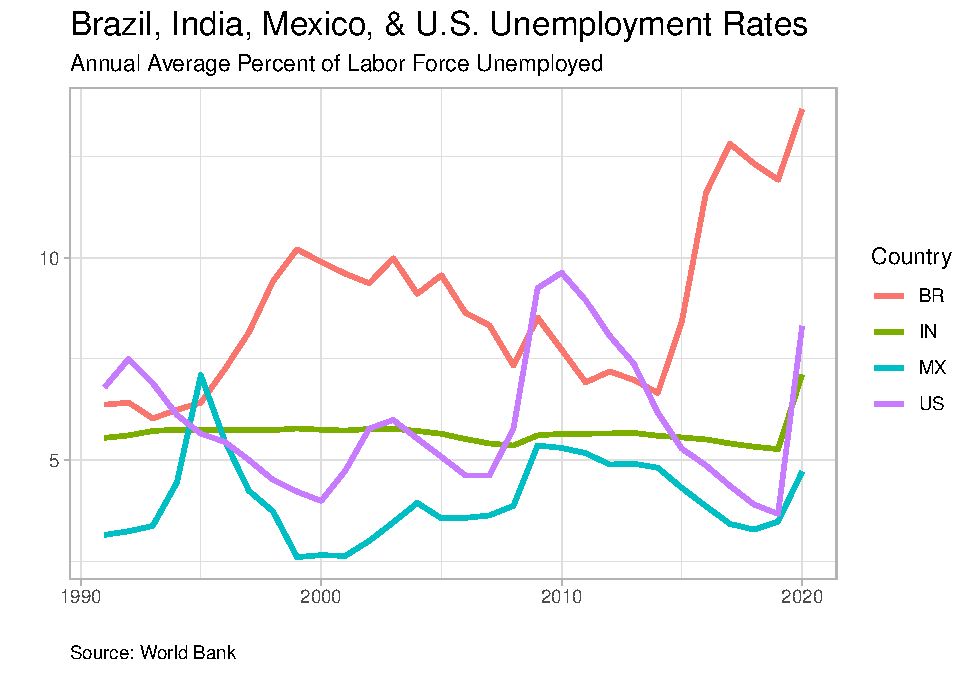
\includegraphics{econ200-book_files/figure-latex/unnamed-chunk-1-1.pdf}

\hypertarget{intro}{%
\chapter{Introduction}\label{intro}}

In Figure \ref{fig:unems} below, you will see the unemployment rate for four countries averaged over each year. The unemployment rate measures the percent of people who cannot find a job in the group of those people either working or looking for work. It seems like a mouthful, but we are estimating the proportion of people who are technically in the \emph{labor force}.

\begin{figure}

{\centering 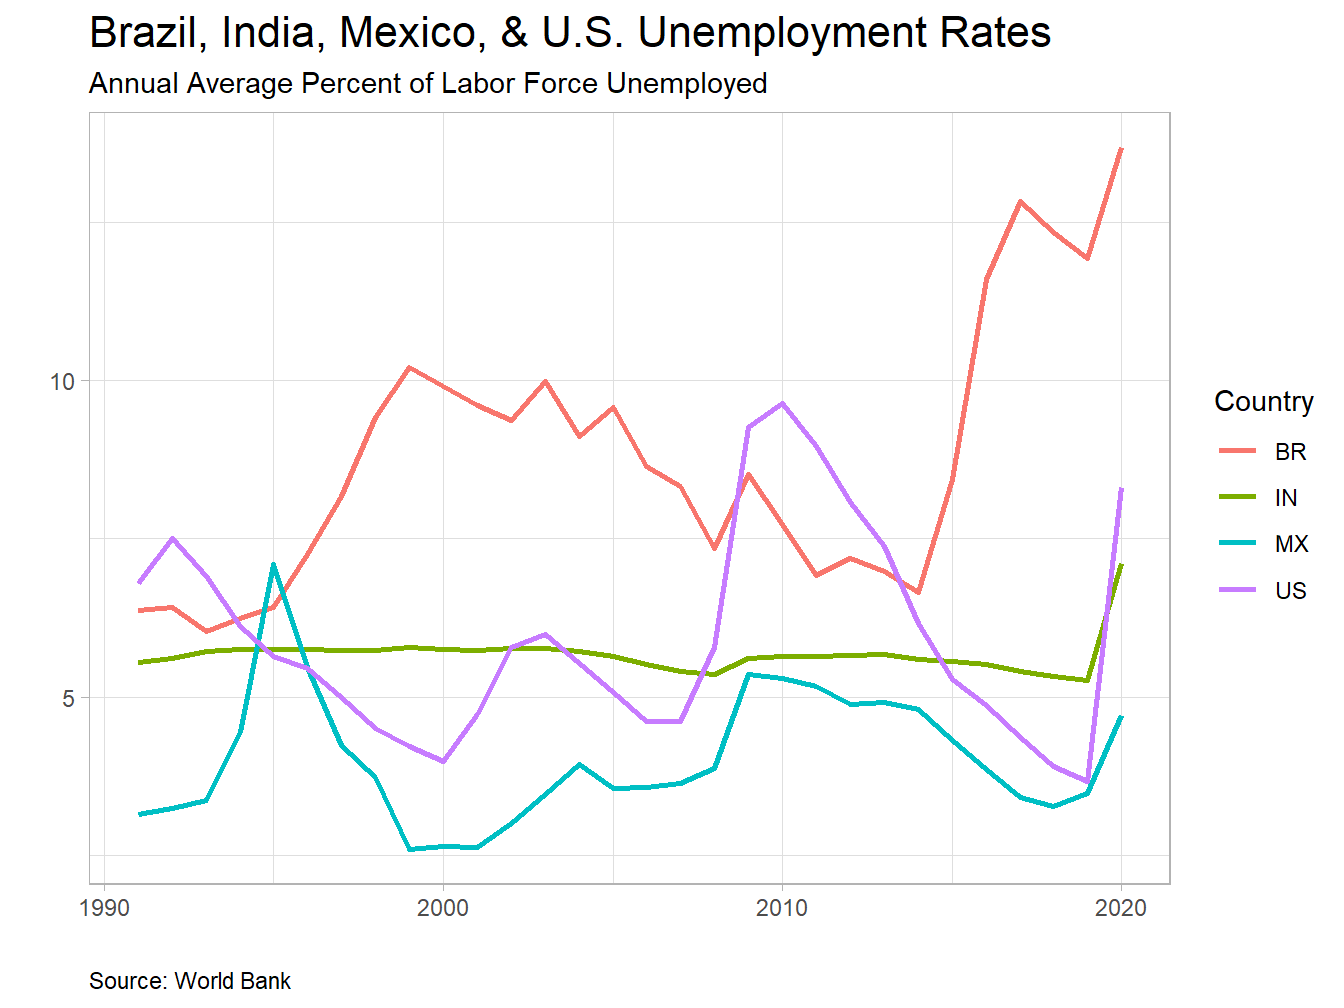
\includegraphics[width=0.8\linewidth]{econ200-book_files/figure-latex/unems-1} 

}

\caption{Unemployment Rates Around the World}\label{fig:unems}
\end{figure}

\begin{quote}
\textbf{Labor Force} is the sum of those who are employed and those actively looking for work.
\end{quote}

We measure the unemployment rate as:

\[ \text{Unemployment Rate} = \frac{\text{Unemployed}}{\text{Unemployed} + \text{Employed}} \times 100 \]

Something important about Figure \ref{fig:unems} is that we can see in some countries the unemployment rate is much higher than in other countries. Partially this is because we do not all use the same measurements for those who are either technically unemployed or working. However, if we assume countries do a consistent job in measuring these rates, the changes are still somewhat accurate. For example, in the United States a monthly survey of about 60,000 households counts those considered unemployed not just as those people collecting unemployment payments, but also includes all those people who have actively sought work in the past four weeks \href{https://www.bls.gov/cps/cps_htgm.htm}{(Bureau of Labor Statistics)}.

In recent months the COVID-19 crisis has gripped the world and put our global economy in a precarious position. As we can see from Figure \ref{fig:jobs} there has been a dramatic increase in the number of people who are newly jobless. Also, other metrics like vehicle miles travelled in the U.S. have crashed dramatically (Figure \ref{fig:vmt}).

\begin{figure}

{\centering 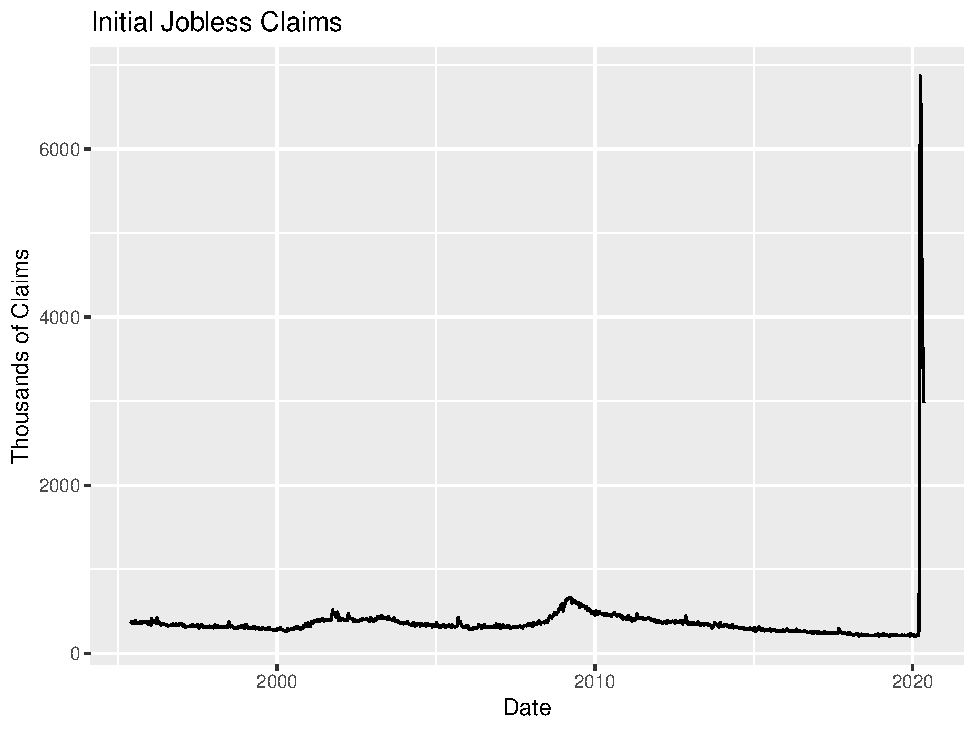
\includegraphics[width=0.8\linewidth]{econ200-book_files/figure-latex/jobs-1} 

}

\caption{Jobless Claims Skyrocket in 2020}\label{fig:jobs}
\end{figure}

\begin{figure}

{\centering 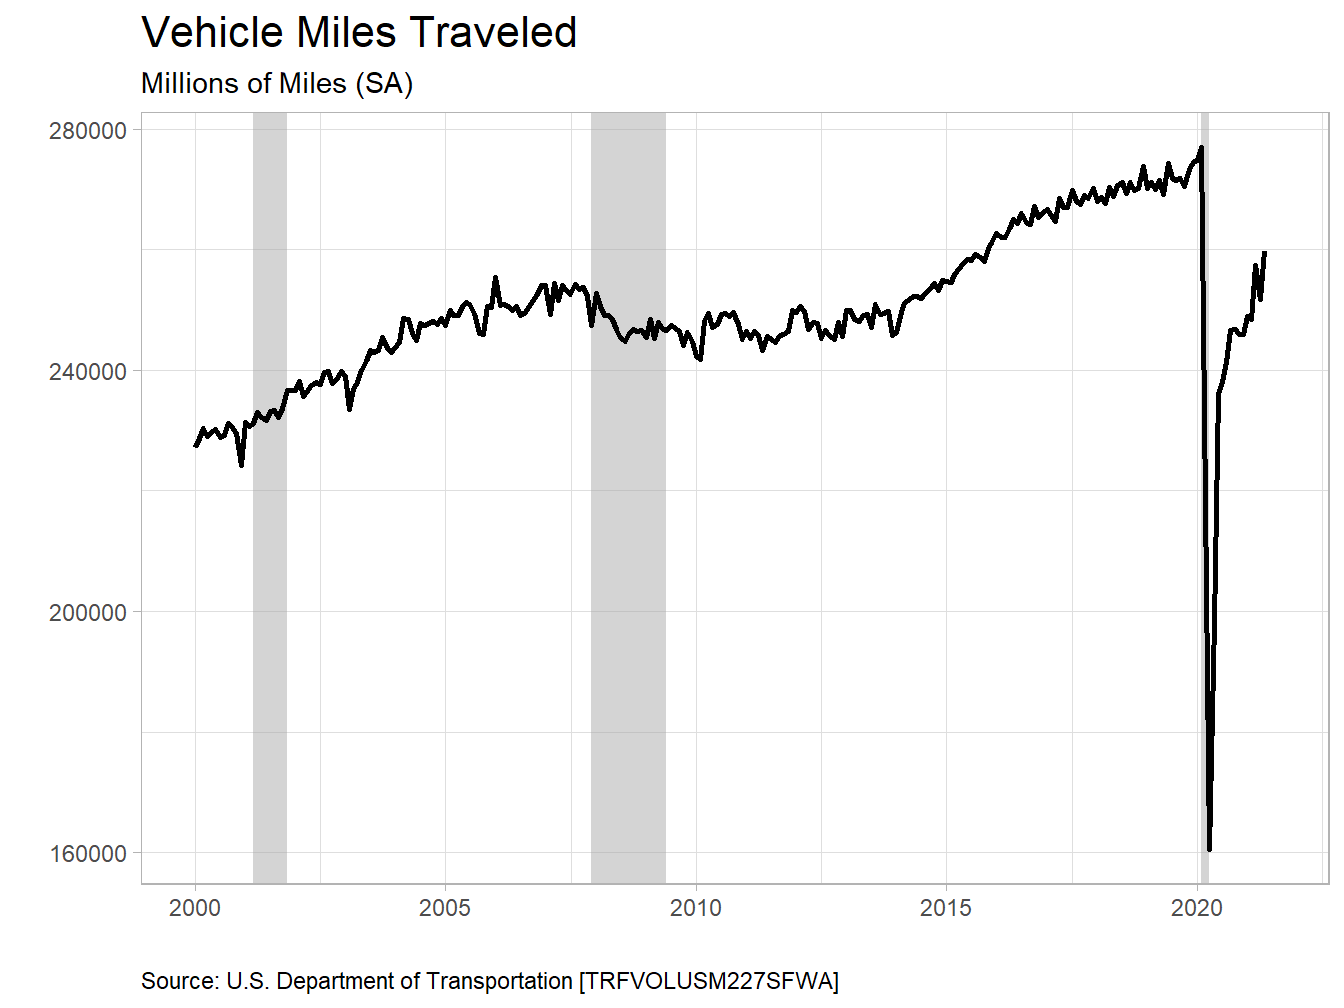
\includegraphics[width=0.8\linewidth]{econ200-book_files/figure-latex/vmt-1} 

}

\caption{Travel Collapses in 2020}\label{fig:vmt}
\end{figure}

Table \ref{tab:initial} shows the initial claims data for the past fifteen weeks, going back to the first weeks of the crisis in early March. Notice that the number of people filing for unemployment rose by a factor of more than ten! These unemployment claim numbers had literally never occurred in the U.S. before.

\begin{table}

\caption{\label{tab:initial}Initial Unemployment Claims for Most Recent 70 Weeks 
 (1000's)}
\centering
\begin{tabular}[t]{lr}
\toprule
Date & Claims\\
\midrule
2020-02-01 & 205\\
2020-02-08 & 207\\
2020-02-15 & 215\\
2020-02-22 & 218\\
2020-02-29 & 216\\
\addlinespace
2020-03-07 & 212\\
2020-03-14 & 256\\
2020-03-21 & 2,923\\
2020-03-28 & 5,985\\
2020-04-04 & 6,149\\
\addlinespace
2020-04-11 & 4,869\\
2020-04-18 & 4,202\\
2020-04-25 & 3,451\\
2020-05-02 & 2,784\\
2020-05-09 & 2,315\\
\addlinespace
2020-05-16 & 2,149\\
2020-05-23 & 1,887\\
2020-05-30 & 1,605\\
2020-06-06 & 1,537\\
2020-06-13 & 1,472\\
\addlinespace
2020-06-20 & 1,460\\
2020-06-27 & 1,436\\
2020-07-04 & 1,398\\
2020-07-11 & 1,479\\
2020-07-18 & 1,398\\
\addlinespace
2020-07-25 & 1,262\\
2020-08-01 & 1,043\\
2020-08-08 & 883\\
2020-08-15 & 920\\
2020-08-22 & 872\\
\addlinespace
2020-08-29 & 875\\
2020-09-05 & 881\\
2020-09-12 & 860\\
2020-09-19 & 860\\
2020-09-26 & 803\\
\addlinespace
2020-10-03 & 782\\
2020-10-10 & 833\\
2020-10-17 & 798\\
2020-10-24 & 768\\
2020-10-31 & 765\\
\addlinespace
2020-11-07 & 728\\
2020-11-14 & 732\\
2020-11-21 & 762\\
2020-11-28 & 719\\
2020-12-05 & 853\\
\addlinespace
2020-12-12 & 873\\
2020-12-19 & 803\\
2020-12-26 & 763\\
2021-01-02 & 781\\
2021-01-09 & 904\\
\addlinespace
2021-01-16 & 886\\
2021-01-23 & 836\\
2021-01-30 & 837\\
2021-02-06 & 863\\
2021-02-13 & 847\\
\addlinespace
2021-02-20 & 747\\
2021-02-27 & 761\\
2021-03-06 & 734\\
2021-03-13 & 765\\
2021-03-20 & 658\\
\addlinespace
2021-03-27 & 729\\
2021-04-03 & 742\\
2021-04-10 & 586\\
2021-04-17 & 566\\
2021-04-24 & 590\\
\addlinespace
2021-05-01 & 507\\
2021-05-08 & 478\\
2021-05-15 & 444\\
2021-05-22 & 405\\
2021-05-29 & 385\\
\bottomrule
\end{tabular}
\end{table}

\hypertarget{money}{%
\chapter{Money \& Banking}\label{money}}

\hypertarget{money-debt-credit}{%
\section{Money, Debt, \& Credit}\label{money-debt-credit}}

Money is an abstract concept, closely linked to the notions of wealth, income, credit, and debt. While most people closely associate money with paper currency issued by governments, it is a much broader social and political construct. As a social construct, money functions as it does---facilitating exchange, measuring value, and storing value---because people agree that it exists. As a political construct, states authorize their money for the payment of taxes and require it to be accepted in payment for debts. In this sense, nations can be considered as the protectors of the debts between occupants of politically delineated boundaries. Money serves several functions. It is a medium of exchange; a unit of account; and a store of value. Money is also a standard of deferred payment.

As a \textbf{medium of exchange} money is not the thing that is consumed in the process of trade but rather a \emph{symbol} of agreed upon value. When a person sells their time to an employer, they are usually paid in money and not tangible consumption goods. The purpose of money in this instance is for the worker to ultimately use it in the future for their own consumption. Thus, there is an implicit agreement upon the value of the goods being exchanged (e.g., labor for time). Money also serves as a \textbf{unit of account}; in that it is how value is measured. In this way, money serves as standard of measurement. Thus, value of objects or actions can be measured and compared to one another. This is much the same as measuring height, weight, or speed. To serve as a \textbf{store of value}, money must retain most of its value over time. If one knew that money had no value at some point in the future, there would be no reason to accept it for exchange today. The store of value represents in some ways the trust that we place in one another when exchanging real things with each other over time.\footnote{\textbf{Real} variables would include things that can be measured objectively, like hiring someone to mow my lawn. The labor it takes to mow the lawn is \emph{real}, as is the machine (i.e., physical capital) used to cut the lawn. The amount of a given currency paid to the worker or to buy the mower is a \textbf{nominal} variable since it is just representing relative value.} Currency issuing nations mandate the terms of payment of taxes, as well as the repayment of debts between a state and its people. Money also serves as a \textbf{standard of deferred payment}. A deferred payment happens when the time of purchase occurs separately from the time of payment. Money serves as the standard with which we value these payments (or debts). Since money represents a standard in inter-temporal commitment (e.g., goods or services are consumed today, but paid for next year), it serves as the object through which our debts and credits are settled with a state or in private transaction.

Money can be used to measure both stock and flow variables. \textbf{Stock variables}---like wealth---are measured at a given point in time. Below, \textbf{balance sheets} represent a typical way of measuring wealth (i.e., net worth) for individuals or capital (i.e., net equity) for companies. \textbf{Flow variables}---like income---are measured over a set length of time. Income might be paid as \$1,000 per week, or \$50,000 per year. Cash flow or income statements are common ways of measuring flow variables.

\textbf{Debt} is a stock concept, representing the sum of obligations owed to others at a given point in time. For example, you might have \$1,200 in accumulated debt at one point in time. \textbf{Deficits} or \textbf{surpluses} are flow concepts represented as the difference between income and expenditures over a set length of time. If you have \$500 a week in income, and \$600 in expenses, the result is a \$100 per-week deficit. In this example, after one week, debt would rise from \$1,200 to \$1,300 as the \$100 deficit is realized. Debts are the accumulated sum of all previous deficits and surpluses. It should be noted that debts do not need to be denominated in terms of an official state-issued currency. You could be in debt to a friend to ``give a ride'', ``move a couch'' or ``buy a drink'' without resorting to dollars or contracts. However, in the U.S., debt is generally measured in dollars. Debt is often inappropriately vilified, when the true concern might be that a person or entity has taken on \emph{too much} debt. It might be better to think of debts as symbolizing promises of future \emph{real} activity. It is common that some person or entity takes on more future real obligations than they might be able to deliver. In this case, when the time comes to collect on an earlier promise which cannot be fulfilled, both the debtor and creditor might renegotiate the terms of repayment.\footnote{Social and political norms can help arbitrate the renegotiation under certain circumstances like death. Suppose a person owes their bank \$1,000, but passes away suddenly. The bank might try to recoup their losses by taking over ownership of the person's house or car.} In most circumstances, debts are repaid. In this way, debt represents the social and community ties that take place over time. It is worth noting that whenever there is a delay in completing a transaction, debts are created. It is nearly impossible to think of a world in which debt does not exist or one where it is outlawed. Hence, debt and money represent a special kind of social contract.

As is explained below, people and banks can create money out of thin air. Today, when an obligation which spans time is entered into between two parties, this debt is measured using money. In this way, a \$10 bill represents future real activity that someone will do for you. Cash, somewhat counterintuitively, is a symbol of debt. If you read a U.S. Federal Reserve Note (U.S. paper money) it says on the front, that ``This note is legal tender for all debts, public and private.'' To the person holding physical or electronic cash, it means either you can repay your debts with it, or you can unlock real activity from someone else by getting them to do something for you. A wealthy individual---like Mark Zuckerberg---holds a great deal of influence over what other people will be doing in the future.

\hypertarget{wealth-and-balance-sheets}{%
\section{Wealth and Balance Sheets}\label{wealth-and-balance-sheets}}

With the concepts of money, debt, and credit introduced, an example can be developed. Imagine that Logan owns several assets. Let's say he has \$1,000 in a checking account, \$60 in cash, a computer he values at \$800, a phone valued at \$500, and a bike worth \$300. These values are what he thinks he can sell these to someone else for. We measure the object's \textbf{liquidity} as the \emph{speed you can turn an asset into cash, without significant loss in value}. Cash and deposits are generally the most liquid assets, since there is minimal risk that it is not worth exactly what you think it is (e.g., \$100 can be sold for \$100). However, a computer, phone, or bike might not sell right away (or ever) at the values you estimate.

We then examine Logan's \textbf{liabilities}, or obligations to others. If he owes \$1,000 to his credit card company, and has \$3,000 in student loans, he has promised to repay those amounts---likely with interest---at some point in the future. We define \textbf{wealth} as the difference between your total asset value and total liabilities. This difference is called wealth or \textbf{net worth} for individuals and \textbf{capital} or \textbf{net equity} for firms and banks. A balance sheet equates total asset value (usually shown on the left-hand side) with total liabilities plus net worth (usually both shown on the right-hand side).

\[ \text{Assets}=\text{Liabilities}+\text{Net Worth}\]

Using these values for the things Logan owns (\$2,660) and debts he owes to others (\$4,000), he would have a net worth of -\$1,340. We need to emphasize that net worth is the item on our balance sheet that \emph{balances} the right-hand and left-hand side of Table \ref{tab:t1}.

\label{tab:t1}\textbf{Logan's Household Balance Sheet}

Assets

Liabilities + Net Worth

Cash

\$60

Credit Card

\$1,000

Deposits

\$1,000

Student Loan

\$3,000

Computer

\$800

Phone

\$500

Bike

\$300

Net Worth

-\$1,340

Total

\$2,660

Total

\$2,660

Having negative wealth does not mean Logan is bankrupt, but it does mean he could not \emph{liquidate} his assets and fully repay his debts. He might be in this situation because he is borrowing money to get an education, investing in his own human capital. He might do this because he expects this human capital investment will pay for itself through additional future earnings, earnings that exceed the amount being borrowed today. Recall, it is only when real promises are unfulfillable that borrowers are in danger of declaring bankruptcy. This arrangement---borrowing money to go to school---is usually a good deal for both the borrower and the lender.

To understand bankruptcy, Logan's cash flow must be considered, as it will show how his wealth is changing over time. Let's assume Logan has an income of \$2,000 per month, with rent of \$800 per month, interest payments of \$50 per month, and other expenses (electricity, cell phone, food, and interest costs on his debt) of \$1,000 per month.\footnote{Note that each of these are flow variables and are comparable since they are measured over the same length of time.} This leaves a surplus of \$150, which we will assume Logan uses \$50 to pay down his credit card debt, \$50 to pay down his student loan debt, and keeps \$50 to add to his checking account.\footnote{For the ease of exposition, interest payments have been combined with all other expenses, and the \$50 per month represents principal repayment.} We write out all the changes to the balance sheet in what is called a \textbf{T-account} which is used to keep track of all the transactions in Table \ref{tab:t2}.\footnote{T-accounts are the flow counterpart of balance sheets, and themselves must balance. When combining a T-account with a starting balance sheet, the changes shown in a T-account will lead you to the updated balance sheet.} Notice that the entire \$150 set aside by Logan to repay debt and increase his checking account balance goes towards increasing his net worth. Some of this occurs through adding to his assets, and some occurs through reducing his liabilities.

\label{tab:t2}\textbf{Logan's Household T-Account for One Month}

Assets

Liabilities + Net Worth

Deposits

\$50

Credit Card

-\$50

Student Loan

-\$50

Net Worth

\$150

Total

\$50

Total

\$50

Our new balance sheet for Logan is visible in Table \ref{tab:t3}, where we can see the changes from our previous balance sheet as described in our T-account.

\label{tab:t3}\textbf{Logan's Updated Balance Sheet}

Assets

Liabilities + Net Worth

Cash

\$60

Credit Card

\$950

Deposits

\$1,050

Student Loan

\$2,950

Computer

\$800

Phone

\$500

Bike

\$300

Net Worth

-\$1,190

Total

\$2,710

Total

\$2,710

\hypertarget{banks-and-money-creation}{%
\section{Banks and Money Creation}\label{banks-and-money-creation}}

Banks can be described using balance sheets and T-accounts in much the same way as we described Logan's personal finances before. Banks are different though in that they are profit-seeking institutions, looking to make money for their investors (i.e., equity holders or shareholders). Interest payments are one form of income for banks, which can lead to bank profits. Banks can also make other profitable investments, such as by buying assets that can be sold for more money than they were purchased for. Interest payments and interest rates are normally described in \emph{nominal} terms. Nominal here just reflects how much more money needs to be repaid in the future and does not dictate how much in additional \emph{real} goods and services are paid by the borrower. Above, we combined interest payments with all other expenses. A person like Logan who owes \$3,000 to a bank for his student loans, with an 11\% annual interest rate, repaid over four years would have to make regular monthly payments of \$77.50, where at first the principal repayment is \$50 and the remaining \$27.50 is interest.\footnote{The \$3,000 is the principal on the loan, the 5\% represents the interest rate, and the four years represents the term to maturity. The \$77.50 figure is found by using an amortization calculator like those found at \url{https://www.amortization-calc.com/loan-calculator/}.} Over the course of the loan, Logan pays \$3,722, which is \$722 in interest, on top of the \$3,000 of principal. At no point does Logan make a big \$3,000 payment, but he instead makes many smaller monthly payments. The same type of calculation would be used for his monthly credit card payments.

Businesses like banks start with capital (i.e., equity or net worth). We start with a group of investors who are opening Jupiter Bank. The owners want to pool some of their financial resources to incorporate as a bank and make a profit. Let's imagine a group of 50 investors who each contribute a \$1,000 cash investment, for a total of \$50,000 as in Table \ref{tab:t4}. The bank starts with a pool of \$50,000 cash.

\label{tab:t4}\textbf{Jupiter Bank Initial Balance Sheet}

Assets

Liabilities + Net Worth

Cash

\$50,000

Capital

\$50,000

Total

\$50,000

Total

\$50,000

As investors, we might think that a big pile of cash is not going generate much of a return. We would be right. If prices rise over time due to inflation, the investors' money buys fewer real goods each year. Investors want their assets to grow over time so that they have greater wealth and can buy more real goods. Thus, the bank owners decide to hire managers who will take some calculated risks on their behalf. To operate as a bank, depositors are needed, and loans would be made. To attract business from people like Logan, the newly founded bank might offer higher interest rates on their deposits than other banks. Let's suppose they offer a 1\% annual return on deposits to Logan, along with a host of other benefits like debit cards, and online banking.

Logan's deposit is a liability to Jupiter, as the bank now owes money to its depositor, Logan. The changes are reflected in a T-account (Table \ref{tab:t5}) and the new balance sheet (Table \ref{tab:t5}).

\label{tab:t5}\textbf{Jupiter Bank: T-Account After Logan's Deposit}

Assets

Liabilities + Net Worth

Cash

\$1,050

Deposits

\$1,050

Total

\$1,050

Total

\$1,050

\label{tab:t6}\textbf{Jupiter Bank: Balance Sheet after Logan's Deposit}

Assets

Liabilities + Net Worth

Cash

\$51,050

Deposits

\$1,050

Capital

\$50,000

Total

\$51,050

Total

\$50,000

\hypertarget{reserves}{%
\section{Reserves}\label{reserves}}

At this point, we will take a closer look at the assets held by Jupiter and give them a new name. What Jupiter had on hand as ``cash'' is called ``reserves'' in banking terminology. The cash is still there, it just has a different name. Banking regulators---like the Federal Reserve in the U.S.---had until recently set up reserve \emph{requirements} which determine \emph{a percentage of deposits that must be held at the bank in the form of cash or on their account with the Fed}. \textbf{Reserve requirements} apply only to deposit accounts, and in the U.S. system banks must maintain a percentage of deposits---on average---over a two-week maintenance period. Since the 1980s, the reserve requirement in the U.S. was technically 10\% for most accounts. Once the COVID-19 crisis took hold though, the reserve requirement was lowered to 0\%, making it such that banks would only hold the amount of reserves they felt necessary.

Banks thus hold \textbf{excess reserves} which are just the amount greater than what they are required to hold.\footnote{Since the reserve requirement is zero, all reserves are considered excess.} Both required and excess reserves are the primary source of liquidity in the banking system. When banks need to meet withdrawals or move money around to other banks, they do it with reserves. Banks generally hold some reserves in the form of \textbf{vault cash}, which is physical currency stored in the bank. Other reserve funds are held electronically on the bank's \textbf{reserve account with the Fed}. The Fed acts as a ``bank for banks'' helping banks transfer money between each other, and they can create reserves out of thin air using a computer keystroke. As is shown below, reserves move with transactions and banks will often borrow them from each other for various reasons. The reserve requirement for this banking system is set at 0\%. With this reserve requirement, the balance sheet can be rewritten, as in Table \ref{tab:t7}. Beginning in October 2008 U.S. banks have been paid interest on their reserve balances. In early 2020, the \textbf{interest rate on reserves} was as high as 1.6\% annually, but was lowered to 0.1\% in late March 2020.\footnote{The Federal Reserve (Fed) pays banks interest on reserves. The Fed creates reserves---out of thin air---to pay to private banks for their reserve balances.} So, with this interest earned on reserves Jupiter Bank is currently getting a positive monthly cash flow simply from offering deposit services to their customers and storing reserve balances. Note, if the Fed were to increase this interest rate, banks would likely want to increase the interest rate that they were charging all their customers who borrow money.

\label{tab:t7}\textbf{Jupiter Bank: Reclassifying Assets from Previous Balance Sheet}

Assets

Liabilities + Net Worth

Required Reserves

\$0

Deposits

\$1,050

Excess Reserves

\$51,050

Capital

\$50,000

Total

\$51,050

Total

\$50,000

At this point, Jupiter Bank's managers decide to purchase some U.S. government bonds (i.e., Treasuries). The return on U.S. Treasuries is low compared to other assets, reflecting the fact that there is very little risk that they will not be repaid. Typically, Treasuries pay a higher interest rate compared to the interest on reserve rate, so here we will assume a 3\% annual return. This higher interest rate is appealing to the bank since it would create more profits for our shareholders. There is also a very liquid market for Treasuries, and it is easy to turn them into cash quickly. Treasuries are also a good source of \textbf{collateral}---an asset pledged by a borrower to a lender, which can be taken and sold if the borrower cannot repay their loan. Good collateral might come in handy if this bank needs to borrow cash. In Table \ref{tab:t8}, we show that Jupiter takes \$20,000 of its cash (i.e., reserves) and uses it to buy some government bonds. These changes are represented in the new balance sheet (Table \ref{tab:t9}).

\label{tab:t8}\textbf{Jupiter Bank: T-Account Due to Securities Purchase}

Assets

Liabilities + Net Worth

Excess Reserves

-\$20,000

Securities

\$20,000

Total

\$0

Total

\$0

\label{tab:t9}\textbf{Jupiter Bank: Balance Sheet after Security Purchase}

Assets

Liabilities + Net Worth

Required Reserves

\$0

Deposits

\$1,050

Excess Reserves

\$31,050

Securities

\$20,000

Capital

\$50,000

Total

\$51,050

Total

\$51,050

Starting from Table \ref{tab:t9}, Jupiter's managers want to make some loans. The interest and fees on the loans made will allow them to pay interest to depositors, finance their operations, and create a profit for the shareholders. Let's assume a potential customer named Olivia wants to borrow \$20,000 to finance a new climbing gym she plans to open. She is willing to borrow the money at an interest rate of 8\%, meaning she would pay about \$1,600 in interest in the first year. When they make her this loan, the bank deposits the funds into an account for her at Jupiter bank so that she can use the money later, paying her the same 1\% rate of return on her deposits that was paid to Logan. Jupiter creates a loan to Olivia, and this transaction is reflected in Table \ref{tab:t10}. Notice the process involves turning reserves into a loan. While somewhat unrealistic, we might imagine this is like Jupiter taking \$20,000 cash from the vault and giving it to Olivia, who promises to repay \$20,000 with interest. She then takes the cash to the teller who takes it and credits her deposit account. Now, think of the deposit as a new transaction. Since the bank is not required to hold any reserves, all \$20,000 that Olivia deposits is considered excess reserves. A more realistic example would be to imagine \emph{electronic claims} to money moving back and forth instead of paper money. In this case, Jupiter might never have even had the cash on hand.

\label{tab:t10}\textbf{Jupiter Bank: T-Account Due to New Loan to Olivia and Her Redeposit}

Assets

Liabilities + Net Worth

Excess Reserves

-\$20,000

Loan

\$20,000

Deposits

\$20,000

Excess Reserves

\$18,000

Total

\$20,000

Total

\$20,000

Jupiter's new balance sheet in Table \ref{tab:t11} has increased by \$20,000 on both sides, just as the T-account described. Note that the bank makes money and loans out of thin air. The loan is an asset to the bank, and while there is a risk that Olivia will not repay, the bankers are willing to take this risk in order to make a profit. On the opposite side of the balance sheet, the deposits Jupiter created are a liability to the bank. Earning a profit relies upon Olivia fulfilling her end of the deal and doing the real work in the future necessary to repay her loan and interest.

Now, imagine that Olivia takes \$1,000 and uses her debit card connected to her deposit account to buy materials for her gym. This moves money out of her deposit account, and a corresponding amount of reserves must go with it. Note, that with the \$1,000 being moved out of the bank, the \$1,000 of excess reserves fall as well.

\label{tab:t11}\textbf{Jupiter Bank: Balance Sheet after Olivia Loan \& Deposit}

Assets

Liabilities + Net Worth

Required Reserves

\$0

Deposits

\$21,050

Excess Reserves

\$31,050

Securities

\$20,000

Loans

\$20,000

Capital

\$50,000

Total

\$71,050

Total

\$71,050

\label{tab:t12}\textbf{Jupiter Bank: T-Account Due to Olivia's Debit Card Use}

Assets

Liabilities + Net Worth

Deposits

-\$1,000

Excess Reserves

-\$1,000

Total

-\$1,000

Total

-\$1,000

\label{tab:t13}\textbf{Jupiter Bank: Balance Sheet after Olivia Uses Debit Card}

Assets

Liabilities + Net Worth

Required Reserves

\$0

Deposits

\$20,050

Excess Reserves

\$30,050

Securities

\$20,000

Loans

\$20,000

Capital

\$50,000

Total

\$70,050

Total

\$70,050

\hypertarget{capital-requirements-and-lending}{%
\section{Capital Requirements and Lending}\label{capital-requirements-and-lending}}

Banks make loans to create profit and pay for the expenses of running their business. Below, we describe why regulators like the Federal Reserve in the U.S. want to ensure that banks have enough capital on hand if some of the banks risky investments do not pan out. The Federal Reserve does this using \textbf{capital requirements} which mandates banks to have a \textbf{capital ratio} that is at least a certain percentage of risky loans. Capital ratios are complicated in practice, but for illustrative purposes we set the capital requirement at 10\% of loans. In Table \ref{tab:t13}, the total amount of loans is \$20,000, and 10\% of this would be \$2,000. The bank, with \$50,000 in capital is well above the \$2,000 requirement. Jupiter's managers are free to make more loans if they wish. They are also meeting their reserve requirement in Table \ref{tab:t13} with \$30,050 in reserves for \$20,050 in deposits. With deposits of \$20,050, they are required to have \$0 in reserves, but they are holding some anyways in the form of excess reserves.

Both the reserve and capital ratio requirements are important in practice. The reserve requirement used to exist to ensure that banks have enough liquidity to meet withdrawals. While capital requirements exist to ensure that banks remain \textbf{solvent} in the event of losses. An \textbf{insolvent} bank would be one who could not liquidate all their assets and repay their liabilities.

Let's imagine that Jupiter makes a new \$40,000 loan to Emma who wants to start a cupcake shop. Emma plans to redeposit this loan in the bank, and like Olivia is also willing to pay an 8\% interest rate on this loan. At the moment the loan is made, the bank does not have enough in excess reserves (since \$30,050 \textless{} \$40,000) and making the loan would leave them with only a portion of the reserves they are required to have. However, because Emma redeposits the money at Jupiter, there is no shortfall in required reserves. You should notice that in this situation, the total amount of reserves between Table \ref{tab:t13} and \ref{tab:t15} is unchanged. In the next section, we discuss what happens if Emma were to write a large check using the newly created deposits just placed in her account.

\label{tab:t14}\textbf{Jupiter Bank: T-Account Due to New Loan to Emma and Her Redeposit}

Assets

Liabilities + Net Worth

Excess Reserves

-\$40,000

Loan

\$40,000

Deposits

\$40,000

Excess Reserves

\$40,000

Total

\$40,000

Total

\$40,000

\label{tab:t15}\textbf{Jupiter Bank: Balance Sheet after Emma's Loan and Redeposit}

Assets

Liabilities + Net Worth

Required Reserves

\$0

Deposits

\$50,050

Excess Reserves

\$30,050

Securities

\$20,000

Loans

\$60,000

Capital

\$50,000

Total

\$110,050

Total

\$110,050

\hypertarget{fed-funds-loans}{%
\section{Fed Funds Loans}\label{fed-funds-loans}}

Let's suppose that Emma wants to hire Cupcake Startup Inc.~to help her get a cupcake shop up and running. Emma writes a check for \$40,000 on her account, paid to Cupcake Startup Inc., who has an account at a different bank (Europa Bank in Table \ref{tab:t17}). When Emma pays Cupcake Startup Inc., money is transferred from one bank to another. Europa Bank's reserves and deposits increase by the amount that they fall at Jupiter Bank.

\label{tab:t16}\textbf{Jupiter Bank: T-Account Due to Emma's Check Writing}

Assets

Liabilities + Net Worth

Deposits

-\$40,000

Excess Reserves

-\$40,000

Total

-\$40,000

Total

-\$40,000

Now, a question is whether Jupiter is still meeting its reserve requirements. In Table \ref{tab:t18}, because of the changes described in Table \ref{tab:t16}, excess reserves are negative. Negative excess reserves indicate a shortfall in reserves. In this case, it can be viewed as total reserves being -\$9,950, with a shortfall of reserves of \$9,950. What should the bank do, given that they are short of their liquidity requirement?

\label{tab:t17}\textbf{Europa Bank: T-Account (Cupcake Startup Inc.'s Bank)}

Assets

Liabilities + Net Worth

Deposits

\$40,000

Excess Reserves

\$40,000

Total

\$40,000

Total

\$40,000

\label{tab:t18}\textbf{Jupiter Bank: Balance Sheet after Emma's Check is Cashed}

Assets

Liabilities + Net Worth

Required Reserves

\$0

Deposits

\$10,050

Excess Reserves

-\$9,950

Securities

\$20,000

Loans

\$50,000

Capital

\$50,000

Total

\$60,050

Total

\$60,050

Jupiter could choose to borrow the funds from another bank on the overnight market. Since Jupiter needs to pay for the funds that they borrow, we will assume that they borrow the smallest amount that they need, or \$9,950. These loans between banks are for terms as short as one night, and banks like Jupiter who are borrowing pay the federal funds rate (or close to it) for this money. Before the COVID-19 pandemic in 2020, the federal funds rate was just below 1.6\%, very near to the interest on reserves rate. After the pandemic caused a lot of problems with the economy, the Fed lowered this interbank loan rate to between 0.00\% and 0.25\%. This interbank loan shows up as a liability to Jupiter, and it is worth noting that it costs them less than deposits (recall we set the rate paid to deposits at 1\% here). Jupiter's borrowing can be seen in the new balance sheet in Table \ref{tab:t20}, which has grown by the amount of the interbank loan. One feature of the federal funds rate market is that the loans are not collateralized, meaning the bank is borrowing reserves from another bank on the promise that the loan will be repaid. If banks cannot get a federal funds market loan, they are often able to post assets (like government securities) as collateral and borrow money at similar rates.

A key feature of the interbank loan market is that banks do not have to hold reserves against these funds. Thus, it is a way banks can meet their requirements without having to maintain additional reserves.

\label{tab:t19}\textbf{Jupiter Bank: T-Account Due to Interbank Loan}

Assets

Liabilities + Net Worth

Interbank Loan

\$9,950

Excess Reserves

\$9,950

Total

\$9,950

Total

\$9,950

\label{tab:t20}\textbf{Jupiter Bank: Balance Sheet after Interbank Loan}

Assets

Liabilities + Net Worth

Required Reserves

\$0

Deposits

\$10,050

Excess Reserves

\$0

Interbank Loan

\$9,950

Securities

\$20,000

Loans

\$50,000

Capital

\$50,000

Total

\$70,000

Total

\$70,000

As long as there are excess reserves somewhere in the system, and other banks believe the borrowing bank is likely to repay, banks have access to necessary funds. If there is a shortfall in reserves---because many banks are trying to borrow---the Fed can ``inject'' liquidity into the system by creating reserves which they can use to temporarily purchase assets like Treasuries from a bank or the general public. They would do this \textbf{open-market purchase} when they observe the federal funds rate---the overnight cost of borrowing---is rising above their preferred \textbf{target federal funds rate}. The target federal funds rate along with the interest rate on reserves are the most important interest rates set by the \textbf{Federal Open Market Committee} during their meetings, which occur every six weeks.\footnote{The FOMC can decide to change rates in between meetings, but this is rare and usually only in response to very severe shocks. The last time the FOMC changed interest rates in between meetings was in early 2008.} The Federal Reserve Open Market Desk purchases securities from the banking system or general public, using reserves that it creates out of thin air. These reserves are usually electronic, but the Fed can direct the Treasury to print paper currency that could also be used as reserves. We assume here in Table \ref{tab:t21} and \ref{tab:t22} that the Fed buys \$10,000 of bonds directly from Jupiter---even if this is an unlikely real-world scenario.\footnote{Notice that the Fed is effectively using newly created money to bid up the price of bonds that are for sale on the open market. This would lead to an increase in the price, and a decline in the interest rate. In our example here, this is what the Fed is trying to accomplish. When interest rates are rising away from the Fed's target federal funds rate, they inject liquidity to ease the upward pressure. If interest rates are falling below their target, their goal is to extract liquidity, lowering prices and raising interest rates.}

In this scenario the Fed is fulfilling its role as the \emph{lender of last resort} and ultimate source of liquidity to the system. If the system is \emph{illiquid} then the creation of credit for borrowers like Olivia might slow down more than anticipated. Credit plays a very important role in our economy, as it helps finance firm operations, and helps smooth consumption by households who otherwise receive lumpy payments.

\label{tab:t21}\textbf{Jupiter Bank: T-Account Due to Open Market Sale of Securities}

Assets

Liabilities + Net Worth

Securities

-\$10,000

Excess Reserves

\$10,000

Total

\$0

Total

\$0

\label{tab:t22}\textbf{Jupiter Bank: Balance Sheet after Open Market Sale of Securities}

Assets

Liabilities + Net Worth

Required Reserves

\$0

Deposits

\$10,050

Excess Reserves

\$10,000

Interbank Loan

\$9,950

Securities

\$10,000

Loans

\$50,000

Capital

\$50,000

Total

\$72,005

Total

\$72,005

\hypertarget{binding-constraints-and-bankruptcy}{%
\section{Binding Constraints and Bankruptcy}\label{binding-constraints-and-bankruptcy}}

Following the Fed's purchase of bonds from Jupiter, we observe that Jupiter can make more loans and still meet its capital and reserve requirements. With \$50,000 in capital, they can make up to \$500,000 in loans, since \$50,000 is 10\% of \$500,000 and 10\% is our capital requirement. Also, with \$10,000 in reserves, they would be able to have an \emph{infinite} amount of deposits---since 0\% is our technical reserve requirement. This does not mean they want to make an infinite amount of loans, just that they are not currently constrained by either requirement. Also note that since Jupiter has access to the overnight market for reserves that they could increase lending and borrow the reserves necessary to meet any requirement. It is worth reiterating that the job of Jupiter bank is to make a profit, and holding onto reserves only earns the interest on reserves rate of 0.1\% paid by the Fed. Let's next presume that the managers of Jupiter target a level of \$150,000 in loans, which are made to customers who redeposit their money back into the bank. Jupiter's balance sheet is now shown in Table \ref{tab:t23}.

\label{tab:t23}\textbf{Jupiter Bank: Balance Sheet after Increasing Loan Portfolio}

Assets

Liabilities + Net Worth

Required Reserves

\$0

Deposits

\$120,050

Excess Reserves

\$12,050

Interbank Loan

\$1,955

Securities

\$10,000

Loans

\$150,000

Capital

\$50,000

Total

\$172,005

Total

\$172,005

To reach the target level of loans of \$150,000, Jupiter would have had to have made \$100,000 in additional loans. This is 10-times the excess reserves in Table \ref{tab:t22}. With these additional loans, let's see if the bank is meeting its capital and reserve requirements. The bank has exactly 10\% of its deposits held as reserves, so it is meeting that requirement since it is above \$0. As for capital, the bank has \$150,000 in loans, and needs to have 10\% (or \$15,000) in capital. The bank has \$50,000, well over \$15,000 in capital required, so the bank is also meeting its capital requirement.

Recall that the act of a bank lending comes with a degree of risk, the risk being that the borrower will not repay the loan. Thus, when banks lend people money to buy homes, they usually require the purchaser to post the house as collateral to the loan as well as put a cash ``down payment'' towards the purchase price. Historically, this down payment was 20\% of the purchase price, so a \$100,000 apartment would require the buyer pay \$20,000 in cash up front. The bank would provide the other \$80,000 in the form of a mortgage. If the borrower loses their job or cannot come up with their mortgage payments, they are \textbf{foreclosed} on by the bank. In foreclosure, the bank seizes the apartment and can resell it to recoup their losses. Since banks do not typically like to own homes, they will often try to sell these homes as fast as possible, likely selling it for less than it might otherwise be worth. In this situation, the bank would face losses on the value of their assets, since they \textbf{write-down} or reduce the value of their loan portfolio.

In Table \ref{tab:t24}, we presume that Jupiter faces losses of \$10,000 on its loans. This might be because the bank lent a client money who ran up a balance on a credit card which they were unable repay and went into bankruptcy. In our balance sheet in Table \ref{tab:t25}, Jupiter's loans and capital decline together. The bank still owes its depositors their money back, and their reserves are not available to reflect losses. The owners of the bank suffer these losses, and the bank's overall balance sheet shrinks.

\label{tab:t24}\textbf{T-Account Due to \$10,000 Write-down on Loan Portfolio}

Assets

Liabilities + Net Worth

Loans

-\$10,000

Capital

-\$10,000

Total

-\$10,000

Total

-\$10,000

\label{tab:t25}\textbf{Balance Sheet after \$10,000 Write-down on Loan Portfolio}

Assets

Liabilities + Net Worth

Required Reserves

\$0

Deposits

\$120,050

Excess Reserves

\$12,050

Interbank Loan

\$1,955

Securities

\$10,000

Loans

\$140,000

Capital

\$40,000

Total

\$162,005

Total

\$162,005

Taking this a step further, now assume that Jupiter has made a lot of bad loans, so many in fact that they lose another \$45,000 in value (Table \ref{tab:t26}). The new balance sheet would show a negative value for net worth in Table \ref{tab:t27}. At this point, Jupiter is \textbf{insolvent}, meaning it cannot liquidate its assets and repay its creditors. The \textbf{Federal Deposit Insurance Corporation} (FDIC) exists to intervene in these circumstances. The FDIC makes depositors whole and makes up for the shortfall in capital at a loss to the FDIC insurance fund. Banks like Jupiter are members of the FDIC and pay periodic insurance premiums to help ensure the solvency of the banking system.

The FDIC usually tries to intervene well before the bank is insolvent, and usually tries to help arrange for another firm to buy the failing firm. Another bank might want to buy access to Jupiter's depositors, their remaining loan portfolio, or the physical locations and employees.

\label{tab:t26}\textbf{T-Account Due to \$45,000 Write-down on Loan Portfolio}

Assets

Liabilities + Net Worth

Loans

-\$45,000

Capital

-\$45,000

Total

-\$45,000

Total

-\$45,000

\label{tab:t27}\textbf{Jupiter Bank: Balance Sheet after \$45,000 Write-down on Loan Portfolio}

Assets

Liabilities + Net Worth

Required Reserves

\$0

Deposits

\$120,050

Excess Reserves

\$12,005

Interbank Loan

\$1,955

Securities

\$10,000

Loans

\$95,000

Capital

-\$5,000

Total

\$117,005

Total

\$117,005

\hypertarget{capital-v.-reserve-constrained-banking}{%
\section{Capital v. Reserve Constrained Banking}\label{capital-v.-reserve-constrained-banking}}

Regulation of both capital and liquidity play an important role in banking. Here we examine another fictional bank---Callisto Bank---to discuss the role for regulation. First, we examine the \textbf{debt-to-equity ratio}, which is calculated as the total amount of liabilities---or debt---to the total amount of capital. In Table \ref{tab:t28}, Callisto Bank has a debt-to-equity ratio of \$210,000 to \$15,000, which is 14-to-1. This is also sometimes referred to as the banks' \textbf{leverage ratio}, since it represents the amount of borrowed money that the bank is using relative to their own capital. Highly leveraged banks are taking more risk, since if the bank's assets decline in value, the losses are amplified by this amount. Next, a \textbf{capital ratio} is found by taking the total of all risky loans, \$120,000, and comparing that to total capital of \$15,000, yielding an 8-to-1 ratio.\footnote{We are assuming here that the debt issued by the bank only takes the form of loans, and equity only comes in the form of capital.} This is the same thing as having 12.5\% of loans held as capital. If we continue using the 10\% requirement from earlier, then this bank is meeting its capital requirement. With \$200,000 in deposits, and \$30,000 in total reserves, the bank is also well above its reserve requirement with a 15\% ratio.

\label{tab:t28}\textbf{Callisto Bank: Balance Sheet}

Assets

Liabilities + Net Worth

Required Reserves

\$0

Deposits

\$200,000

Excess Reserves

\$30,000

Interbank Loan

\$10,000

Securities

\$75,000

Loans

\$120,000

Capital

\$15,000

Total

\$225,000

Total

\$225,000

So, our question is to see how much lending this bank could do and still meet both statutory requirements. With existing reserves, the bank could support an infinite amount of deposits, since \$30,000 of reserves could support any size of deposits (Table \ref{tab:t29}). If we added a \$100,000 loan here, the new balance sheet would have an increase of \$100,000 on each side since the \$30,000 of excess reserves would still be on hand after the increase in deposits.\footnote{Note again, we are assuming all loans created are immediately held as deposits.}

If we check the capital requirement, we will see that the bank is holding loans that place it at more risk than regulators would prefer. Callisto's capital ratio is only at 6.8\% (\$15,000/\$220,000), below its 10\% requirement of \$22,000. Callisto should not be making loans in this amount. In this case, we say they are \textbf{capital constrained} but not \textbf{liquidity constrained}. If Callisto wanted to increase lending while still meeting their capital requirement, they could increase lending from \$120,000 in Table \ref{tab:t30} to \$150,000 (which is \$15,000 divided by the capital requirement of 10\%). The balance sheet would grow by \$30,000. Banks like Callisto might be able to borrow more reserves on the overnight market and increase their lending by much more than the amounts mentioned here. Banks face other regulations, but the role played by capital is very important to understanding the financial crisis in the late 2000s.

\label{tab:t29}\textbf{Callisto Bank: Balance Sheet with Proposed Loan Expansion Based on Reserve Requirement}

Assets

Liabilities + Net Worth

Required Reserves

\$0

Deposits

\$300,000

Excess Reserves

\$30,000

Interbank Loan

\$10,000

Securities

\$75,000

Loans

\$220,000

Capital

\$15,000

Total

\$325,000

Total

\$325,000

Table \ref{tab:t30} is more representative of the modern system, where banking operations are more constrained by access to capital and capital requirements than reserve or liquidity requirements. After the 2008 Financial Crisis, the Federal Reserve increased reserves in the system by nearly \$4 trillion. This increase spurred fears of an overwhelming increase in lending, but those predictions failed to understand that banks were already constrained by capital requirements and a lack of demand for new lending. Following the housing crisis which started in 2006, bank capital had been decimated. Banks were not necessarily eager to go out and make lots of new loans just because they were given the reserves to do so. Instead, they faced much tighter oversight of their capital when many banks were facing a crisis of solvency. The Fed can only do so much when banks face solvency issues, since that is left to the FDIC who does not typically help recapitalize banks. Banks were left to raise capital on their own and were under pressure to find investors who would be willing to give banks money in exchange for ownership stakes in now undercapitalized banks. In 2008, the Troubled Asset Relief Program or TARP authorized the government purchase of an ownership stake in financial institutions that were deemed systemically important. These institutions were effectively nationalized as the government took a large controlling stake in the banks. The government did not overwhelmingly restrict the banking operations of these institutions, although TARP did come with some additional oversight responsibility.

\label{tab:t30}\textbf{Callisto Bank: Balance Sheet with Proposed Loan Expansion Based on Capital Requirement}

Assets

Liabilities + Net Worth

Required Reserves

\$0

Deposits

\$230,000

Excess Reserves

\$30,000

Interbank Loan

\$10,000

Securities

\$75,000

Loans

\$150,000

Capital

\$15,000

Total

\$255,000

Total

\$255,000

\hypertarget{federal-reserve-toolsinstruments-targets-and-goals}{%
\section{Federal Reserve Tools/Instruments, Targets, and Goals}\label{federal-reserve-toolsinstruments-targets-and-goals}}

There is a distinction between the Federal Reserve's tools (or instruments), targets, and goals. The main tools used by the Federal Reserve are the:

\begin{itemize}
\tightlist
\item
  \textbf{Open Market Operations}: The Fed's purchase (sale) of bonds intended to decrease (increase) the federal funds rate. These operations are done multiple times per day with the intention of trying to maintain the Fed's target federal funds rate.
\item
  \textbf{Interest on Reserves}: Starting in October 2008, the Fed began paying banks for holding reserves. There are separate rates paid for required and excess reserves (although they have been set equal to each other since the program's inception). Since 2008, this rate has been used to help guide the federal funds target rate.
\item
  Reserve Requirements: The percentage of deposits that must be held in the form of the bank's reserves.
\item
  \textbf{Balance Sheet Operations}: When the Fed increases the size (quantitative) or quality (qualitative) of its own balance sheet. This can be used to try and influence interest rates other than the federal funds rate.
\item
  \textbf{Discount Rate}: The cost of borrowing reserves directly from the Federal Reserve. This is nearly identical to how the interbank loans work, except the reserves are coming from outside the private sector and the loans are collateralized. There is also an increase in reserves through a discount rate loan.
\end{itemize}

The Fed's targets are the intermediate things the Fed is trying to change which might influence economic activity like consumption or investment. Some examples of targets are the:

\begin{itemize}
\tightlist
\item
  \textbf{Federal Funds Rate}: The Fed sets a target rate in this market by providing sufficient liquidity to push lending conditions towards their preferable state. This interest rate is now guided by the interest on reserves rate which is set to be close to the target fed funds rate. Increases (decreases) to these interest rates are expected to indirectly cause other interest rates to rise throughout the economy, including Treasury and riskier assets.
\item
  \textbf{Long-term Interest Rates}: The Fed might choose to also try to manipulate longer-term interest rates to affect behavior in other markets.
\item
  \textbf{Money Supply}: The Fed could try to target the total supply of money, in the form of deposits and currency (i.e., M1) or the broader M2 money supply (M1+MMMF+Savings+Time deposits).\footnote{Savings accounts or money-market deposit accounts (MMDA) are less liquid than checking. Money market mutual funds (MMMF) are another less-liquid alternative to deposits. Finally, small-denominated time deposits-or certificate of deposit (CDs)-are investments that can be liquidated with a small penalty.}
\end{itemize}

Ultimately, the Federal Reserve is trying to reach its goals of:

\begin{itemize}
\tightlist
\item
  \textbf{Full Employment}: interpreted as unemployment at or near the natural rate of unemployment
\item
  \textbf{Stable Prices}: interpreted as a stable and low rate of inflation at or near 2\%.
\end{itemize}

The Fed is free to change its instruments, and form its own targets, but the goals are more rigid since they are mandated by Congress. By law, the Fed's job is to maintain full employment and stable prices, but they are free to interpret what this means. So, there is some flexibility here, where rather than focus on keeping prices constant they have chosen to instead try to keep inflation steady (which is the rate of change in prices).

\hypertarget{an-aside-on-money-supply}{%
\section{An Aside on Money Supply}\label{an-aside-on-money-supply}}

At times in the past, the supply of money has been debated as an important measure to focus on. In recent years though central banks like the Federal Reserve and European Central Bank have let it be known that the supply of money is not as important as it was once thought to be. This does not mean that pundits and journalists do not emphasize it though, and it often arises in popular media. In early 2020, you can see one measure of the money supply rises very rapidly (Figure \ref{fig:money}). Many people directly attribute this to some response by the Federal Reserve, however the story is a bit more nuanced.

\begin{figure}

{\centering 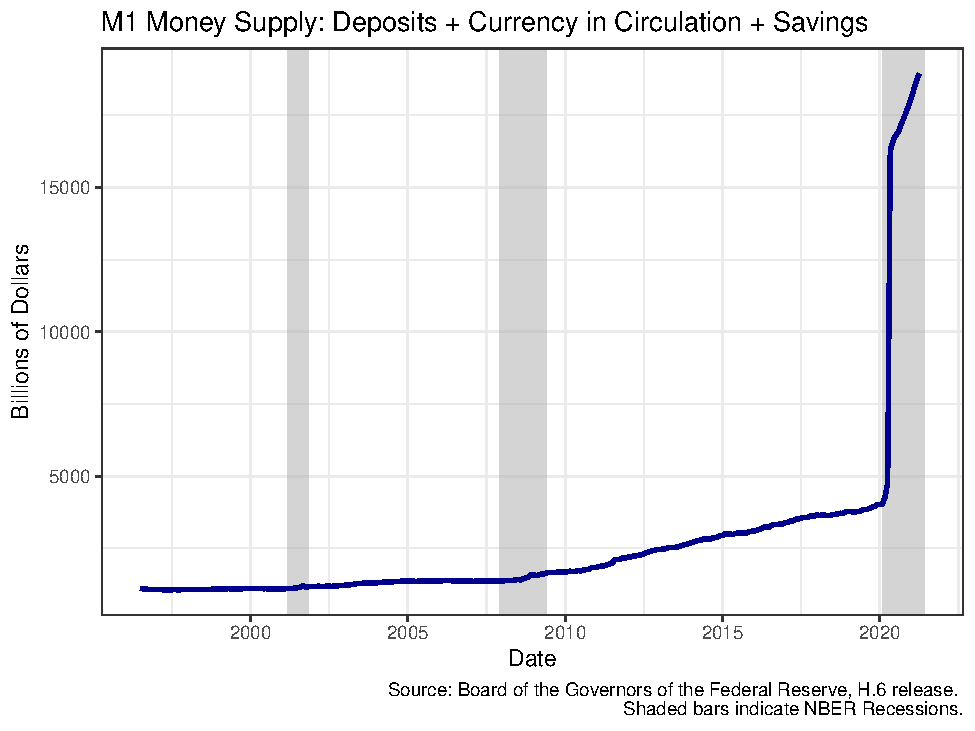
\includegraphics[width=0.8\linewidth]{econ200-book_files/figure-latex/m1-1} 

}

\caption{The M1 Money Supply Has Grown Over Time}\label{fig:m1}
\end{figure}

The measure of money we are observing in Figure \ref{fig:m1} is known as \textbf{M1}. M1 is known as the most liquid form of money. If you look up a definition of M1 in most textbooks or on the internet, you will see it has long been defined as seen in equation \eqref{eq:M1}, which I will call \emph{Old M1}.

\begin{equation}
\text{Old } M1 = \text{Currency in circulation} + \text{Deposits} \label{eq:M1}
\end{equation}

A broader measure of the money supply known as \textbf{M2} was long defined as seen in equation \eqref{eq:M2}---or \emph{Old M2}---and displayed in \ref{fig:M2}. You might note that there is an increase in both M1 and M2 in 2020 during the COVID-19 pandemic, but the increase in M2 is much less pronounced.

\begin{equation}
\text{Old } M2 = M1 + \text{MMMF} + \text{Savings Deposits} + \text{CDs} \label{eq:M2}
\end{equation}

The components of M2 here include all of M1, as well as: \textbf{money market mutual funds} (MMMF)---similar to checking accounts with some restrictions on the ability to withdraw your money; \textbf{Certificates of deposit} (CDs)---also known as small-time deposits typically face a penalty for early withdrawal; and \textbf{savings deposits}, which are often linked to checking accounts and had long had many restrictions on the ability to access your money. Savings accounts are the most important thing to focus on here. The main difference between M1 and M2 here is that there was a technical change in what counted as M1 and M2. As mentioned above, M1 had been defined as in \eqref{eq:M1}, but in March 2020 the Fed eliminated certain restrictions on moving money in and out of savings accounts, thus making them more liquid. The Fed therefore reclassified savings to be part of M1. Importantly, this change does not impact the size of M2.

\begin{figure}

{\centering 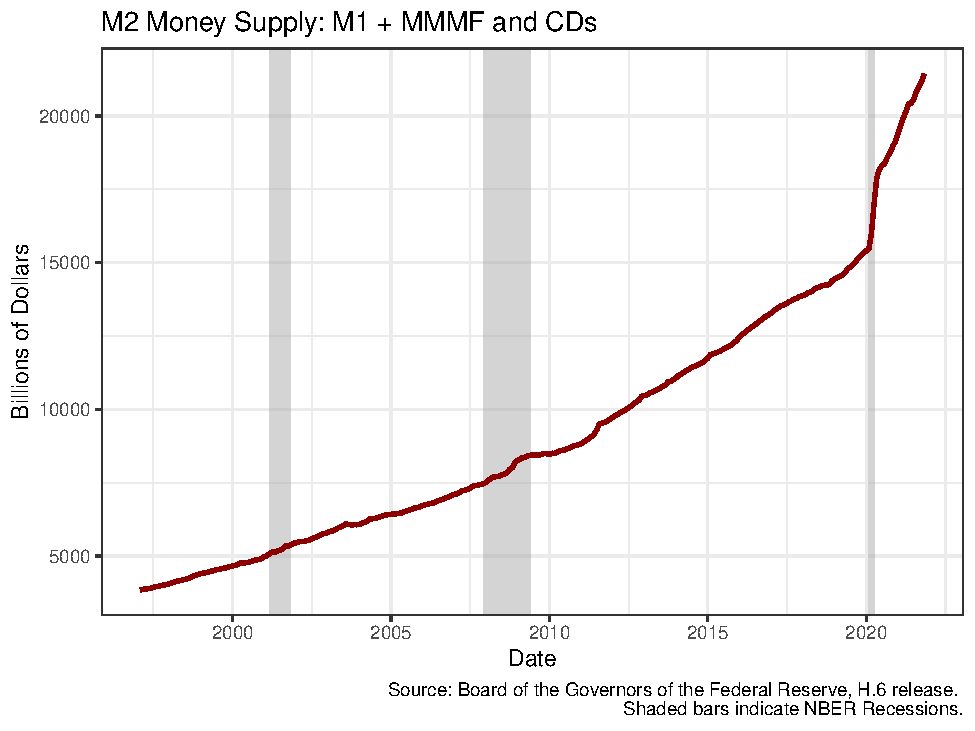
\includegraphics[width=0.8\linewidth]{econ200-book_files/figure-latex/M2-1} 

}

\caption{The M2 Money Supply Has Also Grown}\label{fig:M2}
\end{figure}

The new form of M1 is now:

\begin{equation}
M1 = \text{Currency in circulation} + \text{Deposits} + \text{Savings Deposits} \label{eq:M1b}
\end{equation}

while M2 is the same since savings moved into M1, which is part of M2.

\begin{equation}
M2 = M1 + \text{MMMF} + \text{Certificate of Deposits} \label{eq:M22}
\end{equation}

\begin{figure}

{\centering 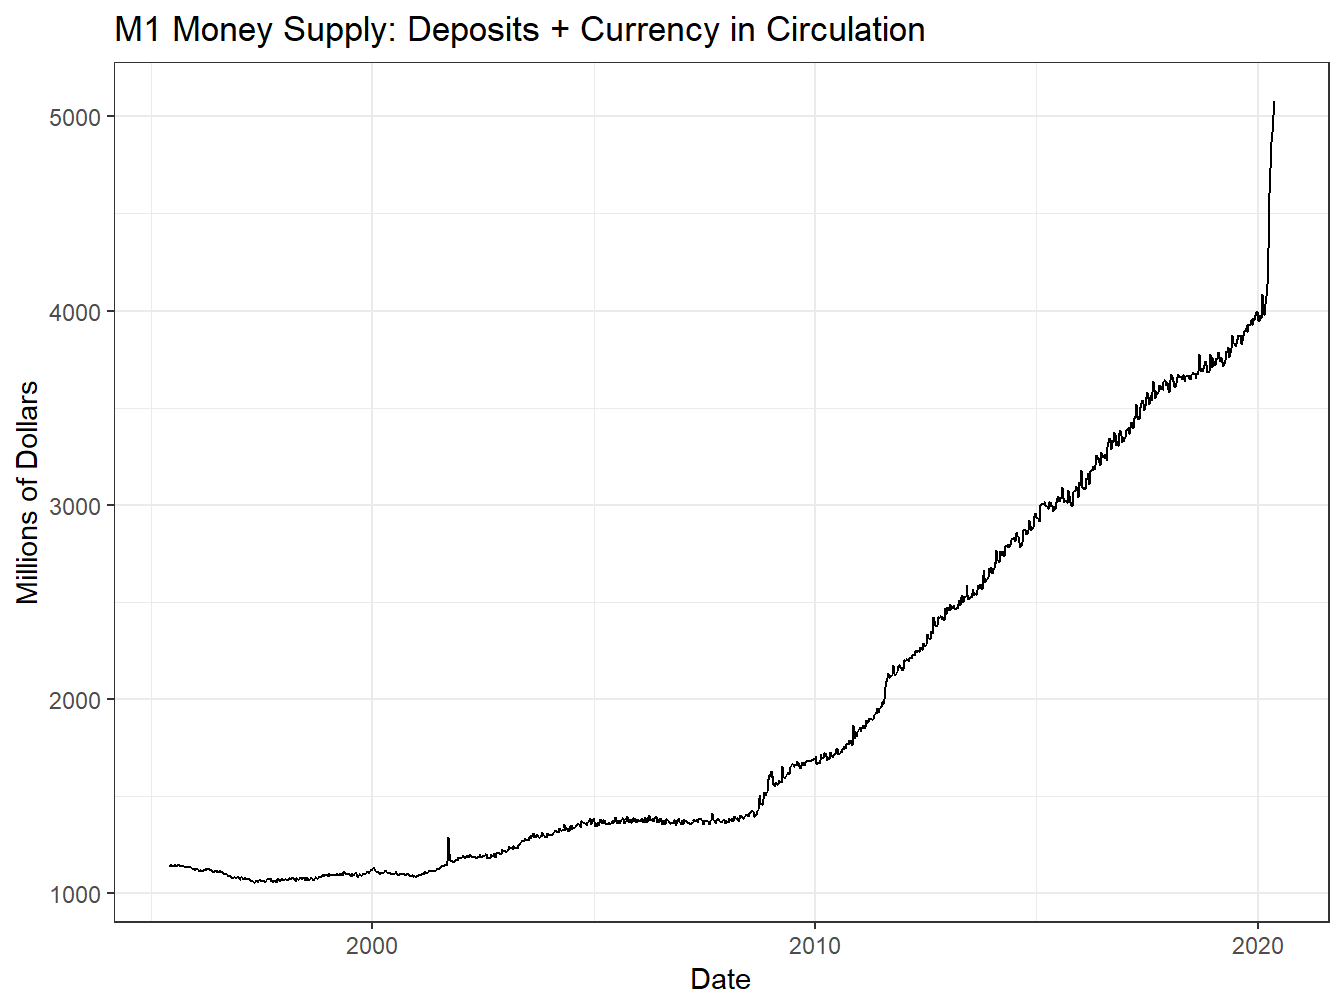
\includegraphics[width=0.8\linewidth]{econ200-book_files/figure-latex/money-1} 

}

\caption{The Money Supply Has Also Changed Over Time}\label{fig:money}
\end{figure}

When plotted together, we can see that if we include savings account balances in the \emph{old M1} definition, that it tracks very closely with M2 until April 2020. Thus, while there are big changes in the COVID-19 pandemic to the various monetary aggregates, the increase in M1 is far less suspicious than some pundits might lead you to believe. The \emph{New M1} series provided by the Fed did not go back and add in savings as I have done here. However, you might now notice that including that aggregate matters for the overall discussion.

With all that said, there is still a big jump in M2 in 2020, and this is due to Fed actions to help rescue the economy during the pandemic. We can see this in another measure of money supply known as the monetary base or \textbf{M0}. Another term to describe M0 is \textbf{outside money} which somewhat confusingly means \emph{money created outside the private banking sector}. We calculate M0 as:

\begin{equation}
M0 = \text{Currency in circulation} + \text{Reserves} \label{eq:M0}
\end{equation}

Seen below in \ref{fig:M0} the monetary base climbed steadily until about 2008 when the U.S. encountered the \emph{financial crisis} related to the bust in the housing market and fallout. The consequences of this crisis were so severe, that the Fed was working to help stimulate the economy and aid the financial system for years to fully recover. Only in the few years prior to 2020 was the monetary base beginning to decline. While some might look at this chart and note that the money supply is rising seemingly without bound, this value of M0 reflects the central bank's efforts to help banks remain liquid throughout a period of crisis.

\begin{figure}

{\centering 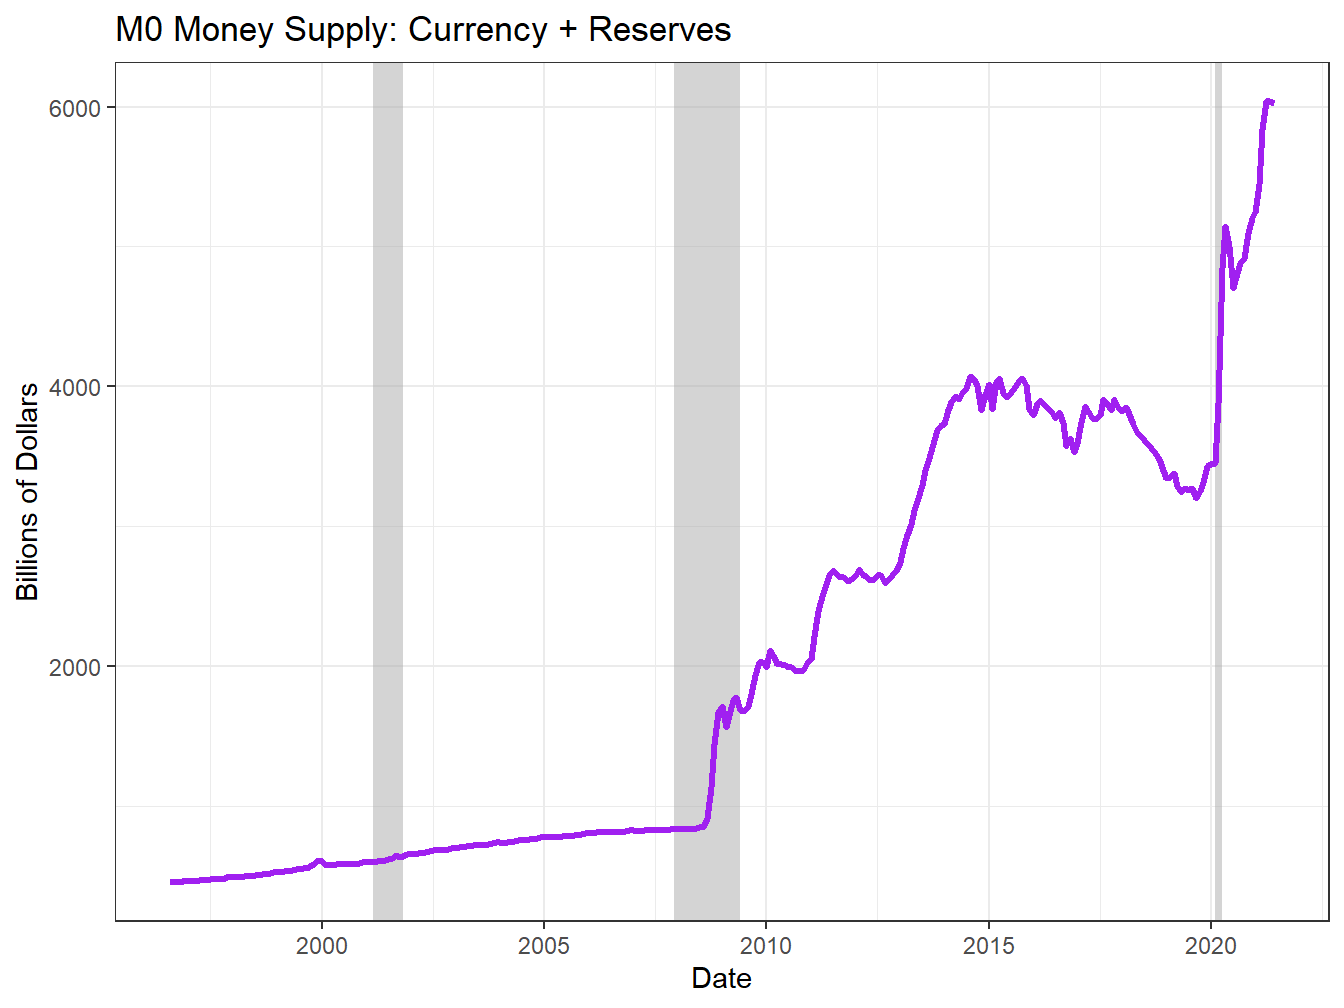
\includegraphics[width=0.8\linewidth]{econ200-book_files/figure-latex/M0-1} 

}

\caption{The Monetary Base Grew During Crises}\label{fig:M0}
\end{figure}

Side-by-side and going back a bit further in time in Figure \ref{fig:moneyfacet}, we can see that there had been a steady increase in M0 and M2 over time, with the 2008 financial crisis being associated with a big change in these aggregates. The next big change occured in 2020 during the COVID-19 pandemic. In the coming chapters, we will discuss the Fed's role a bit more.

\begin{figure}

{\centering 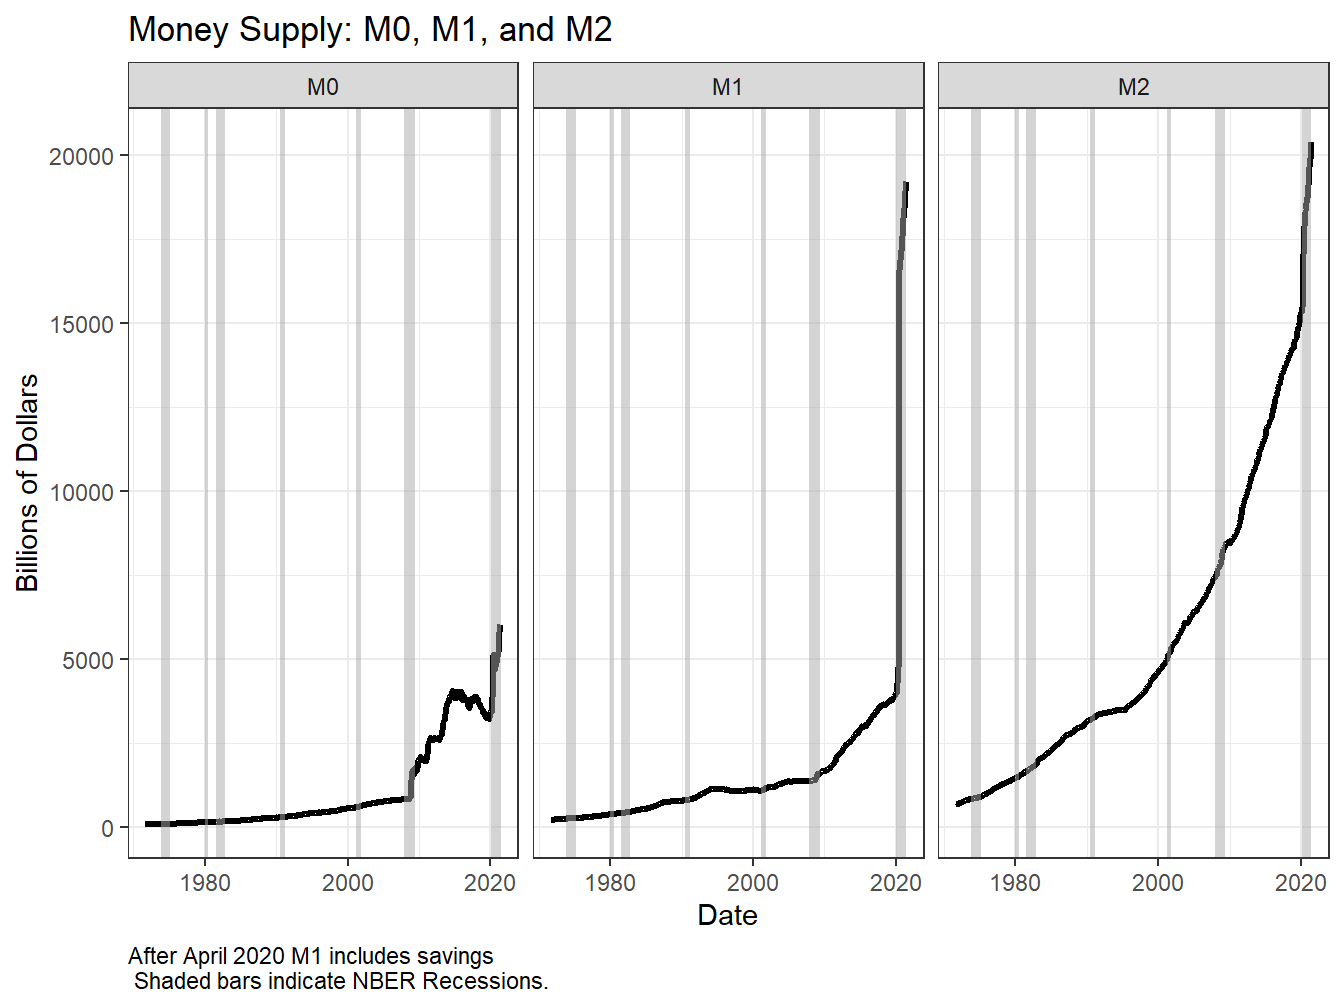
\includegraphics[width=0.8\linewidth]{econ200-book_files/figure-latex/moneyfacet-1} 

}

\caption{Side by Side of Monetary Aggregates}\label{fig:moneyfacet}
\end{figure}

\hypertarget{labor}{%
\chapter{Labor Market Measures}\label{labor}}

\hypertarget{labor-force-participation}{%
\section{Labor Force Participation}\label{labor-force-participation}}

The labor market is one of the most important and relevant macroeconomic measures of health.\footnote{Many of the graphs here are adapted from code available from Len Kiefer's blog post \url{http://lenkiefer.com/2018/03/11/charting-jobs-friday-with-r/}.} There are several different measures of labor market health. First, we might like to know what portion of eligible workers are engaged in either working or job search. We measure this using the \textbf{labor force participation rate} (LFP). The LFP tends to rise and fall with long-term economic trends, like women entering the workforce or the reduction in manpower necessary for manufacturing. We calculate the LFP as:

\[ \text{LFP} = \frac{\text{Unemployed}+\text{Employed}}{\text{Eligible Population}} \times 100 \]

We can see that structural forces shift labor force participation (Figure \ref{fig:labor1}). However, LFP does change with cyclical events, such as the case with the recent COVID-19 pandemic.

\begin{figure}

{\centering 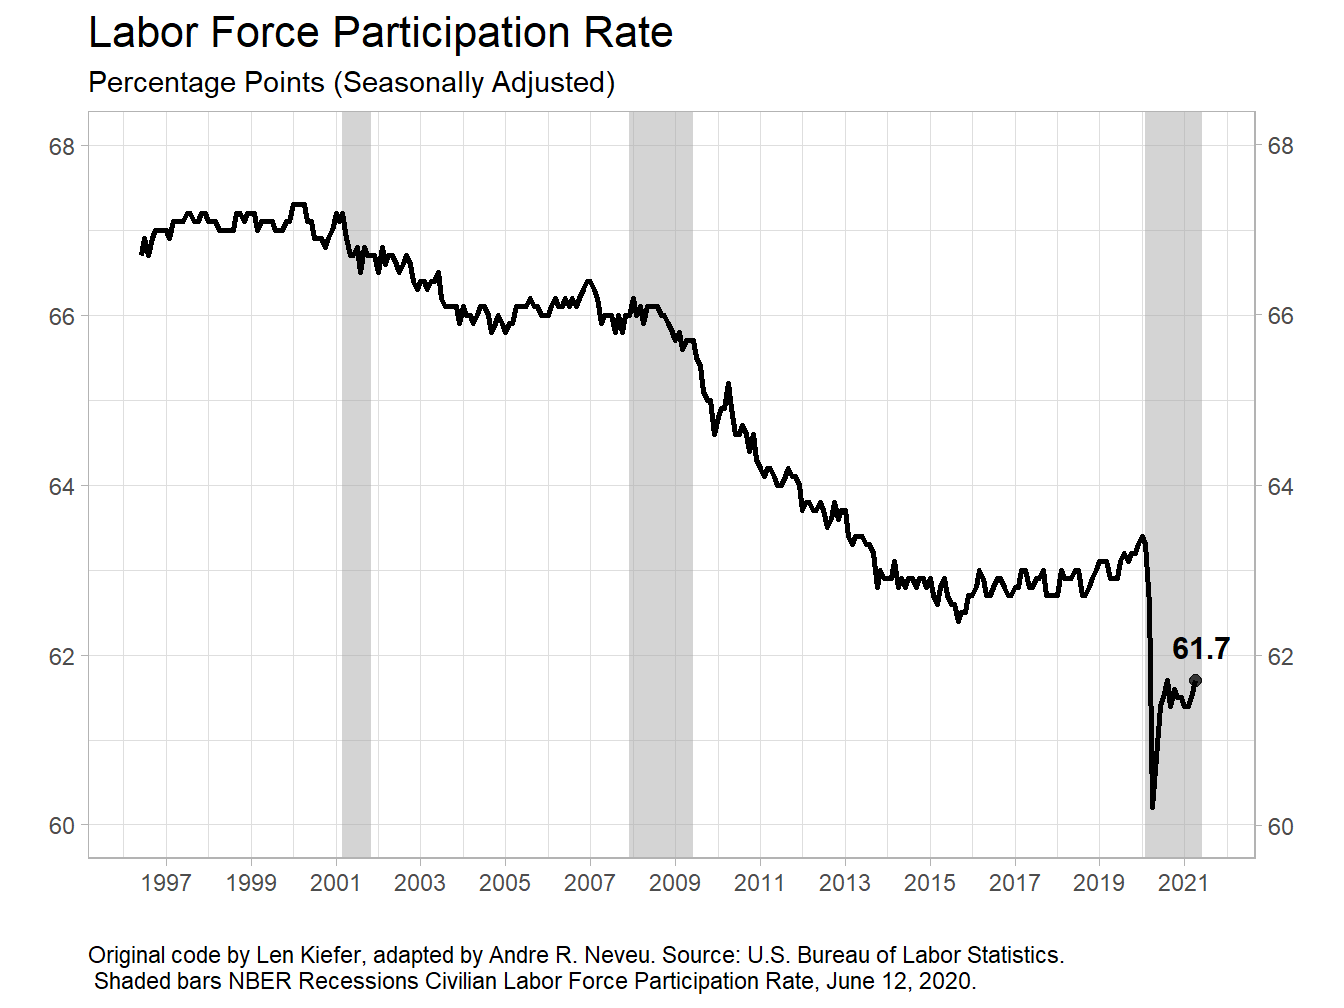
\includegraphics[width=0.8\linewidth]{econ200-book_files/figure-latex/labor1-1} 

}

\caption{The Workforce Shows Structural and Cultural Changes}\label{fig:labor1}
\end{figure}

\hypertarget{job-growth}{%
\section{Job Growth}\label{job-growth}}

Another way to look at the health of the labor market is to look at job growth. Job growth in the U.S. had been going very strong until the COVID-19 pandemic in early 2020. Note that in Figure \ref{fig:neat} there had been positive gains in growth for over ten years! Prior to the COVID-19 pandemic, healthy job growth was considered to be about 200,000 jobs per month.

\begin{figure}

{\centering 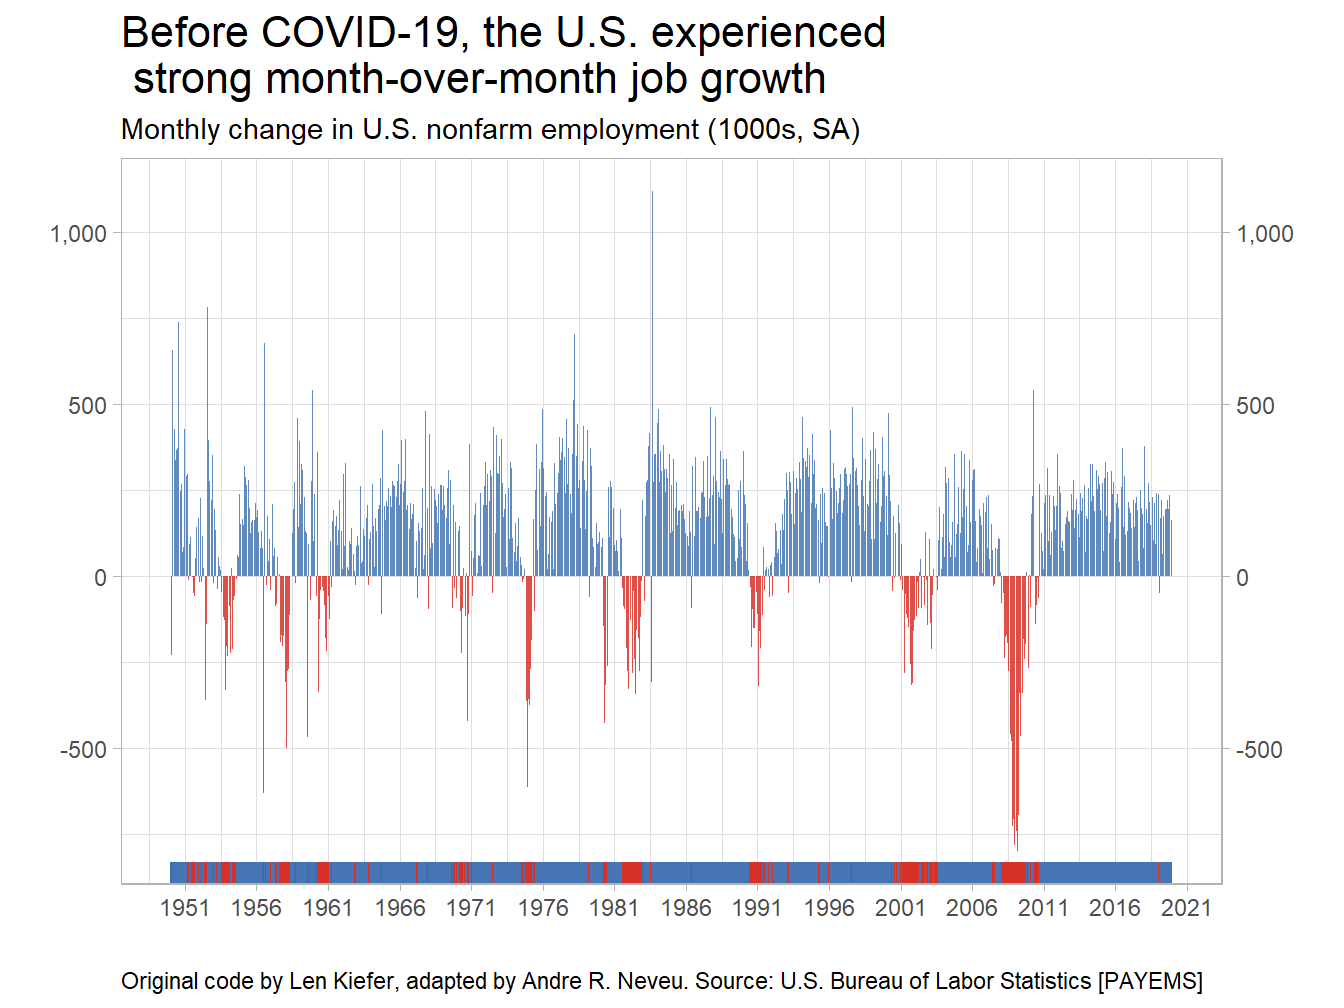
\includegraphics[width=0.8\linewidth]{econ200-book_files/figure-latex/neat-1} 

}

\caption{Job Gains Had Persisted for a Historically Long Stretch}\label{fig:neat}
\end{figure}

The COVID-19 pandemic is unlike anything we have ever experienced in the U.S., so much so that the scale of all previous changes appear nearly irrelevant. Note that Figure \ref{fig:neat2} is the same as Figure \ref{fig:neat} but focuses on the periods since the start of the Great Recession in late 2007.

\begin{figure}

{\centering 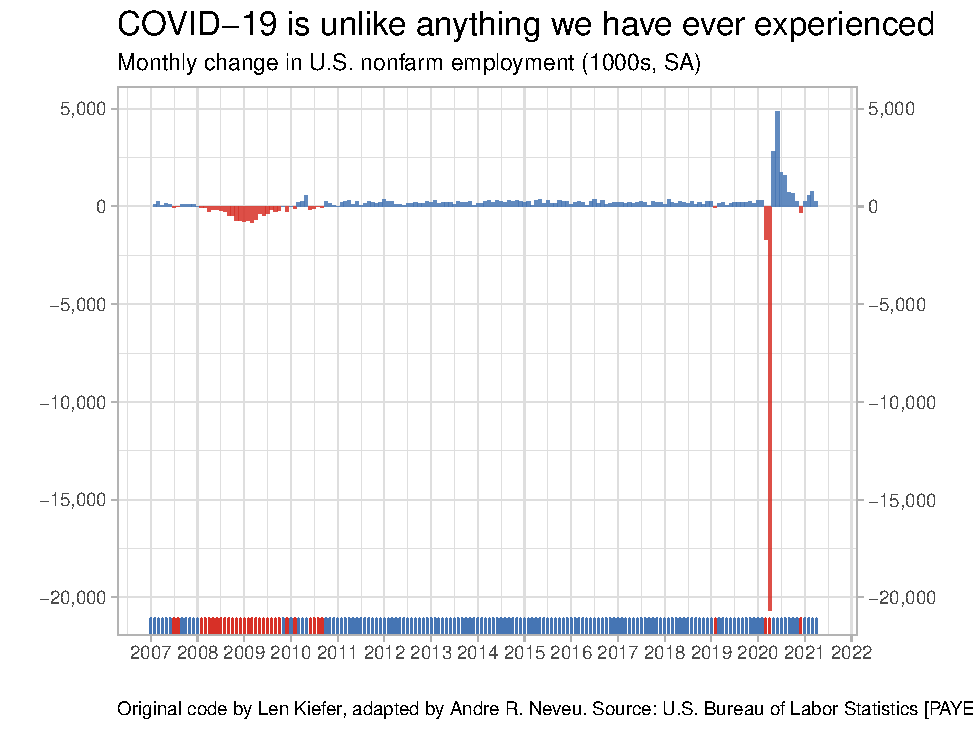
\includegraphics[width=0.8\linewidth]{econ200-book_files/figure-latex/neat2-1} 

}

\caption{The COVID-19 Job Losses Are Stunning}\label{fig:neat2}
\end{figure}

\hypertarget{unemployment-rates}{%
\section{Unemployment Rates}\label{unemployment-rates}}

The unemployment rate is a different measurement than labor-force participation. Unemployment rates only look at the percentage of the labor force that cannot find work. The labor force is the numerator in the calculation of the LFP, and sometimes when people lose a job they leave the labor force entirely. This complicates our perception of the health of the labor market when some people are both losing jobs--leaving the numerator of the unemployment rate--and also leaving the labor force. In mid-2020, people are both filing for unemployment--which means they stay in the labor force--and dropping out of the labor force.

\[ \text{Unemployment Rate} = \frac{\text{Unemployed}}{\text{Unemployed} + \text{Employed}} \times 100 \]

The unemployment rate is often compared to a conceptual measure known as the \textbf{natural rate of unemployment}. This natural rate is what economists estimate the unemployment rate would have to be in order to keep the economy producing at it's potential. \textbf{Potential output} is somewhat confusing, as it really means the country is producing goods and services at a \emph{sustainable} level and not the \emph{absolute maximum}. You might think of potential output more like a pace you could sustain while jogging, but not an all-out sprint! The estimated natural rate of unemployment considers what we have talked about so far. Strong participation, healthy job growth, and availability of jobs making for a \emph{healthy} labor market.

We can see in Figure \ref{fig:neat3} that the unemployment rate in early 2020 was at an historic low, and was well below what economists considered \emph{natural}. When the economy is not doing so well, the labor market tends to be one of the most important signals. Thus, the unemployment rate usually rises rapidly during \textbf{recessions} when the economy and output is contracting.

\begin{figure}

{\centering 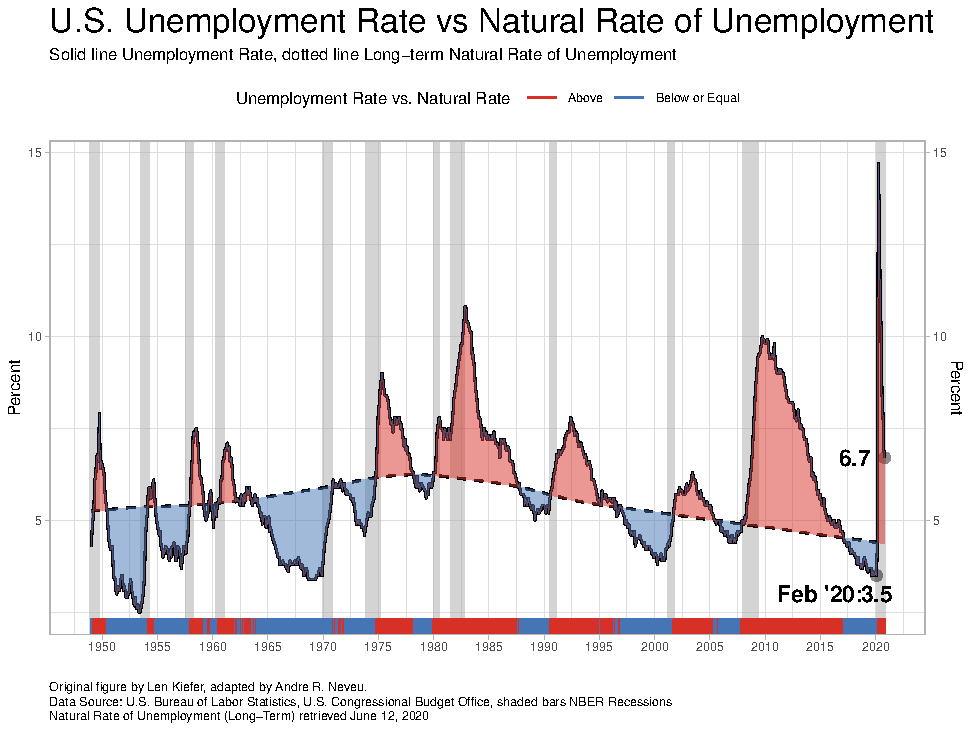
\includegraphics[width=0.8\linewidth]{econ200-book_files/figure-latex/neat3-1} 

}

\caption{Unemployment Rates Had Been Historically Low}\label{fig:neat3}
\end{figure}

\hypertarget{long-run-trends-v.-short-run-changes}{%
\section{Long-Run Trends v. Short-Run Changes}\label{long-run-trends-v.-short-run-changes}}

\begin{figure}

{\centering 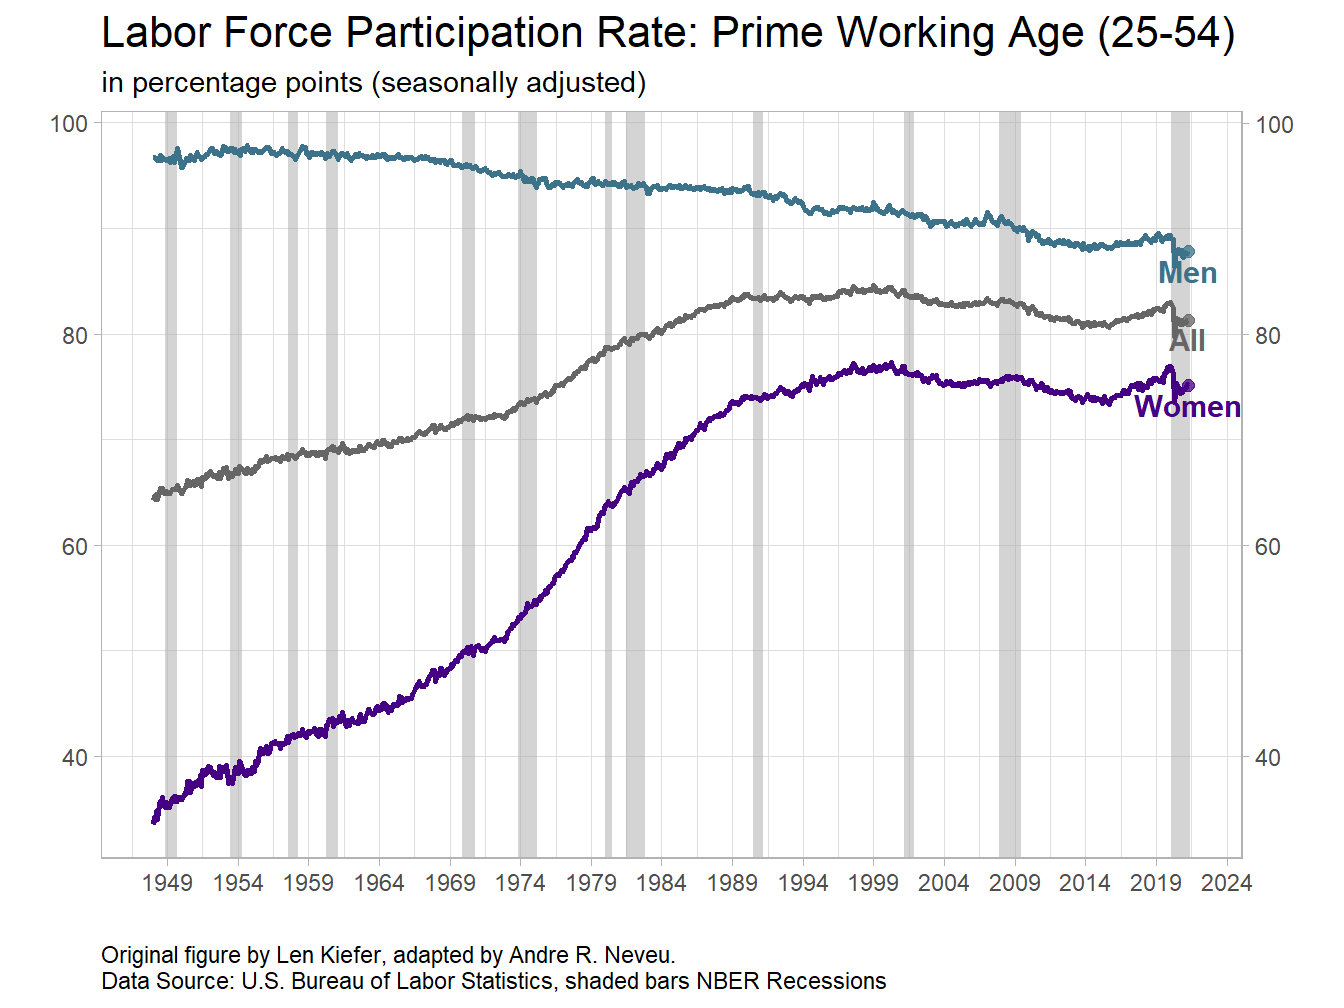
\includegraphics[width=0.8\linewidth]{econ200-book_files/figure-latex/neat5-1} 

}

\caption{Labor Force Participation Has Plummeted}\label{fig:neat5}
\end{figure}

\begin{figure}

{\centering 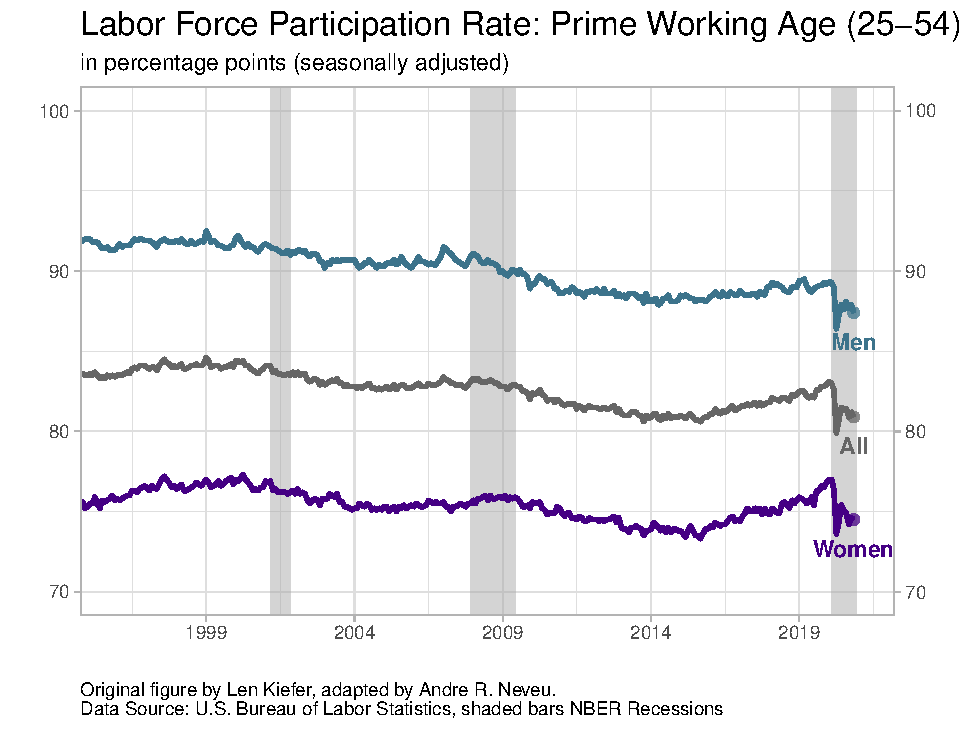
\includegraphics[width=0.8\linewidth]{econ200-book_files/figure-latex/neat6-1} 

}

\caption{The Change is Simiilar Across Gender}\label{fig:neat6}
\end{figure}

\begin{figure}

{\centering 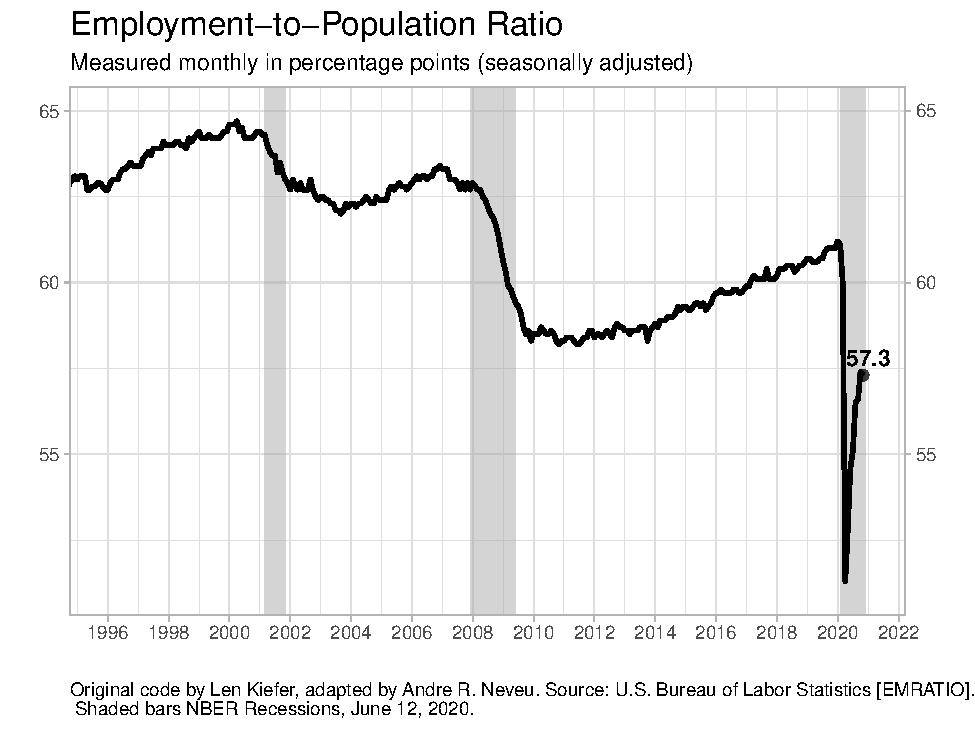
\includegraphics[width=0.8\linewidth]{econ200-book_files/figure-latex/neat7-1} 

}

\caption{Expectedly, the Percentage of All People Employed Has Fallen}\label{fig:neat7}
\end{figure}

\hypertarget{inflation}{%
\chapter{Inflation}\label{inflation}}

Prices for the goods and services we consume change over time. Recall that a price that you pay for a good is simply a \emph{nominal} value, and does not directly take into account the amount of \emph{real} work that would be performed to purchase a good. For example, if you were living in the fictional country of Titan, and a bag of chips there cost 30 units, that information is not particularly informative by itself. First, you want to know if ``30 units'' is a lot. If a typical wage for an hour of work was ``3 units'' then chips seem expensive costing you about 10 hours of work! However, if a typical wage was ``300 units'' for an hour of work, then chips are cheap, earned with about six minutes of work! Thus, what is most important to you is the real value.

For many goods--like tuition--the price level just seems to rise over time. Here, we see the average price \textbf{level} for the U.S. as measured by the \textbf{Consumer Price Index} (CPI). By itself, the CPI in Figure \ref{fig:cpi1} is not particularly informative. In April 2020, the CPI measured 255.902. What we might be more interested in is the change in the CPI, or inflation seen in Figure \ref{fig:cpi2}. So if we look at the CPI from April 2019 when it measured 254.943, we could see that it increased by:

\[\left(\frac{255.902}{254.943} - 1\right)\times 100 = 0.4\%\]

\begin{figure}

{\centering 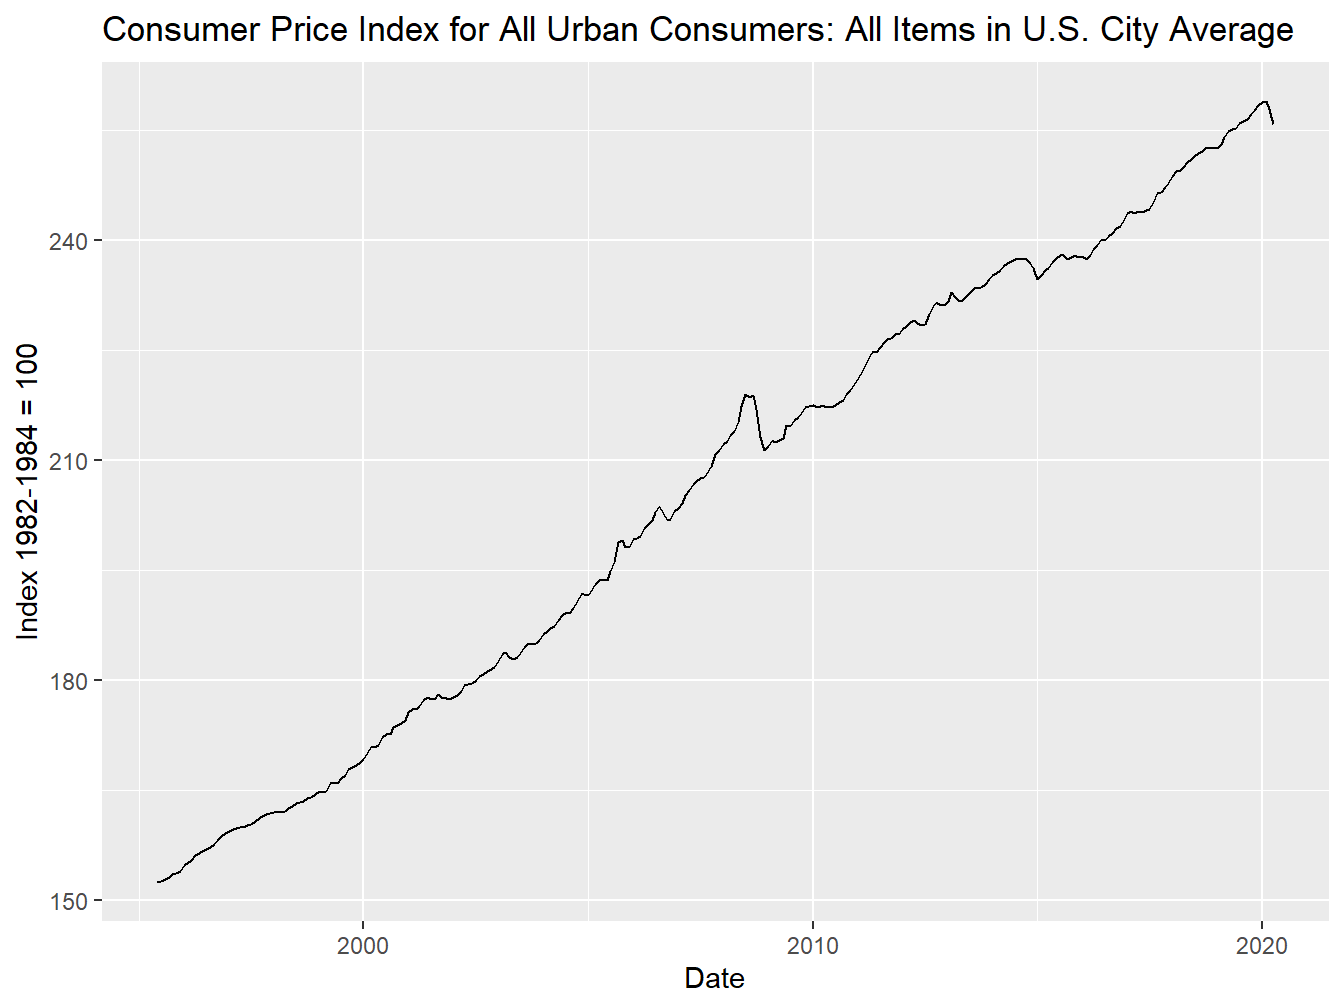
\includegraphics[width=0.8\linewidth]{econ200-book_files/figure-latex/cpi1-1} 

}

\caption{Price Levels Generally Rise Over Time}\label{fig:cpi1}
\end{figure}

\begin{figure}

{\centering 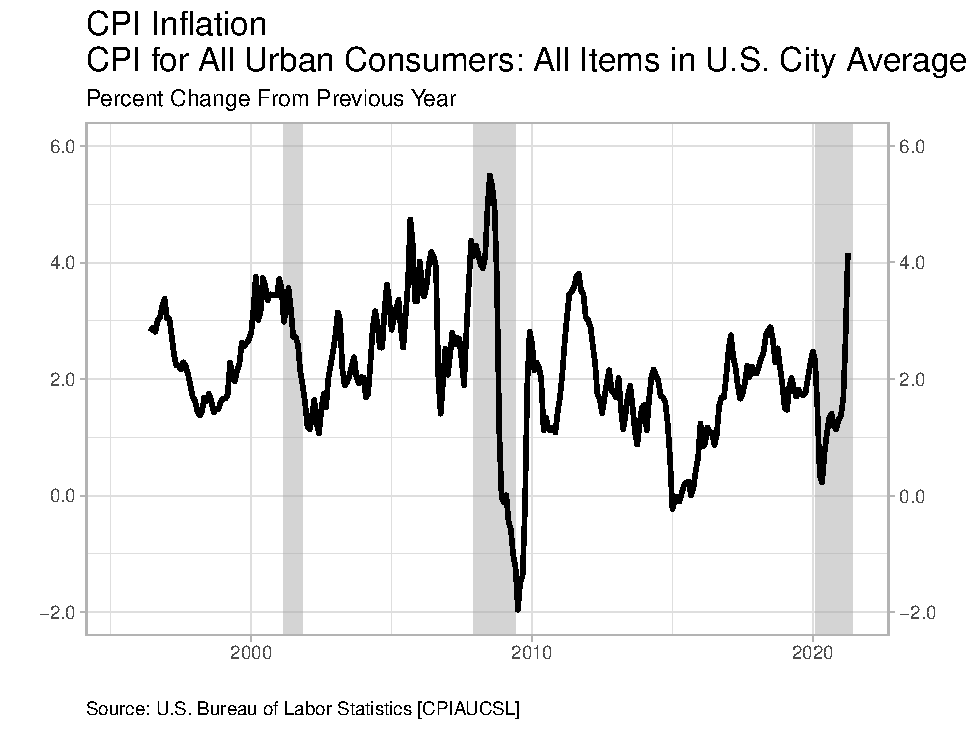
\includegraphics[width=0.8\linewidth]{econ200-book_files/figure-latex/cpi2-1} 

}

\caption{Inflation Rates Are Measuring the Change in the Price Level}\label{fig:cpi2}
\end{figure}

\hypertarget{production}{%
\chapter{Output and Production}\label{production}}

Measures of output and production

\begin{figure}

{\centering 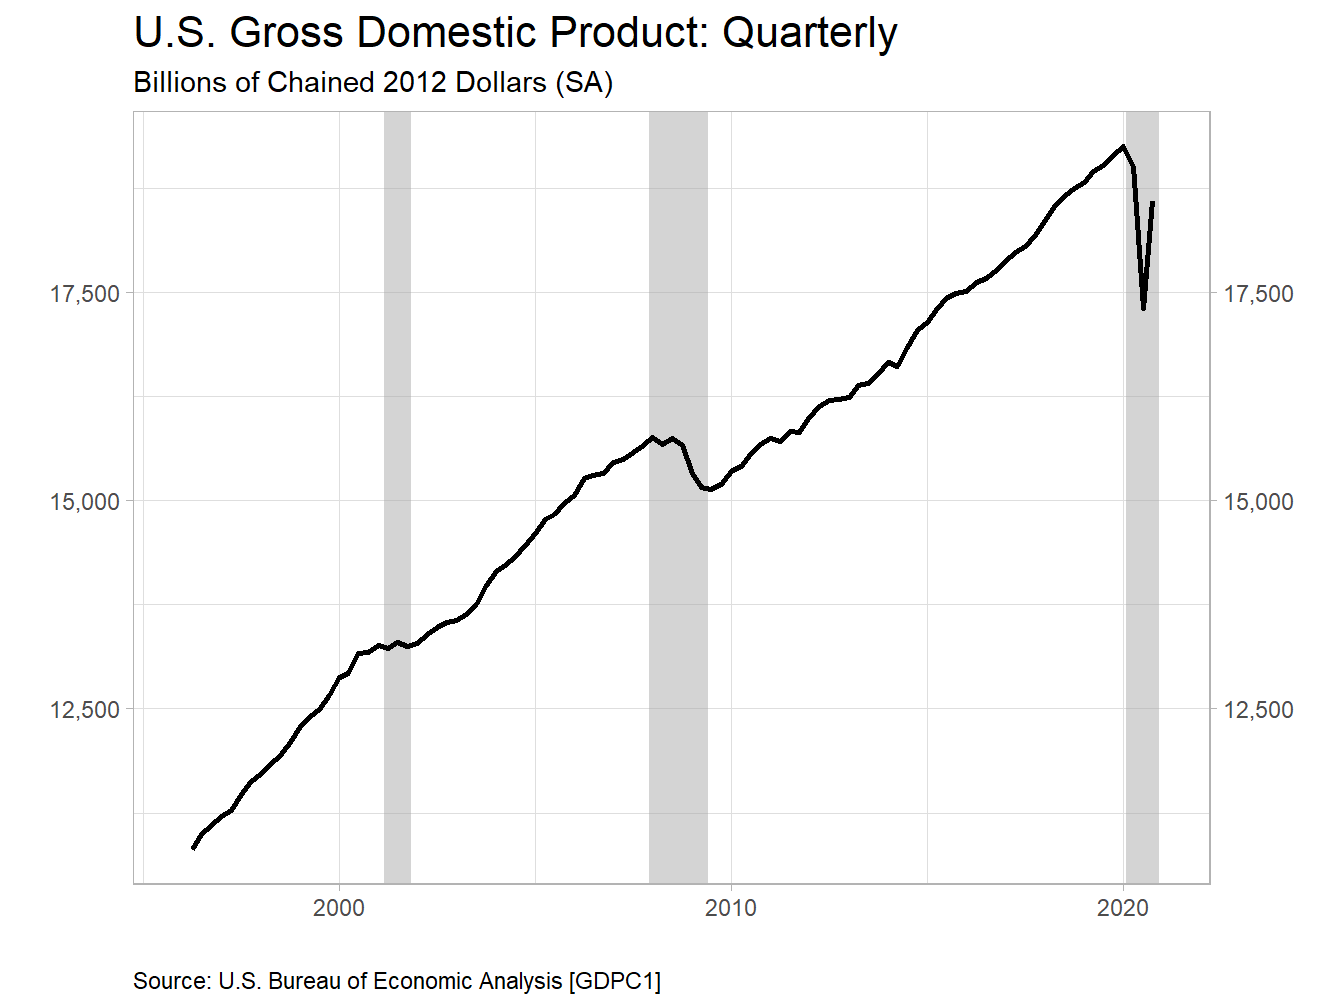
\includegraphics[width=0.8\linewidth]{econ200-book_files/figure-latex/output-1} 

}

\caption{Output Exhibits Both Growth and Cycles}\label{fig:output}
\end{figure}

\begin{figure}

{\centering 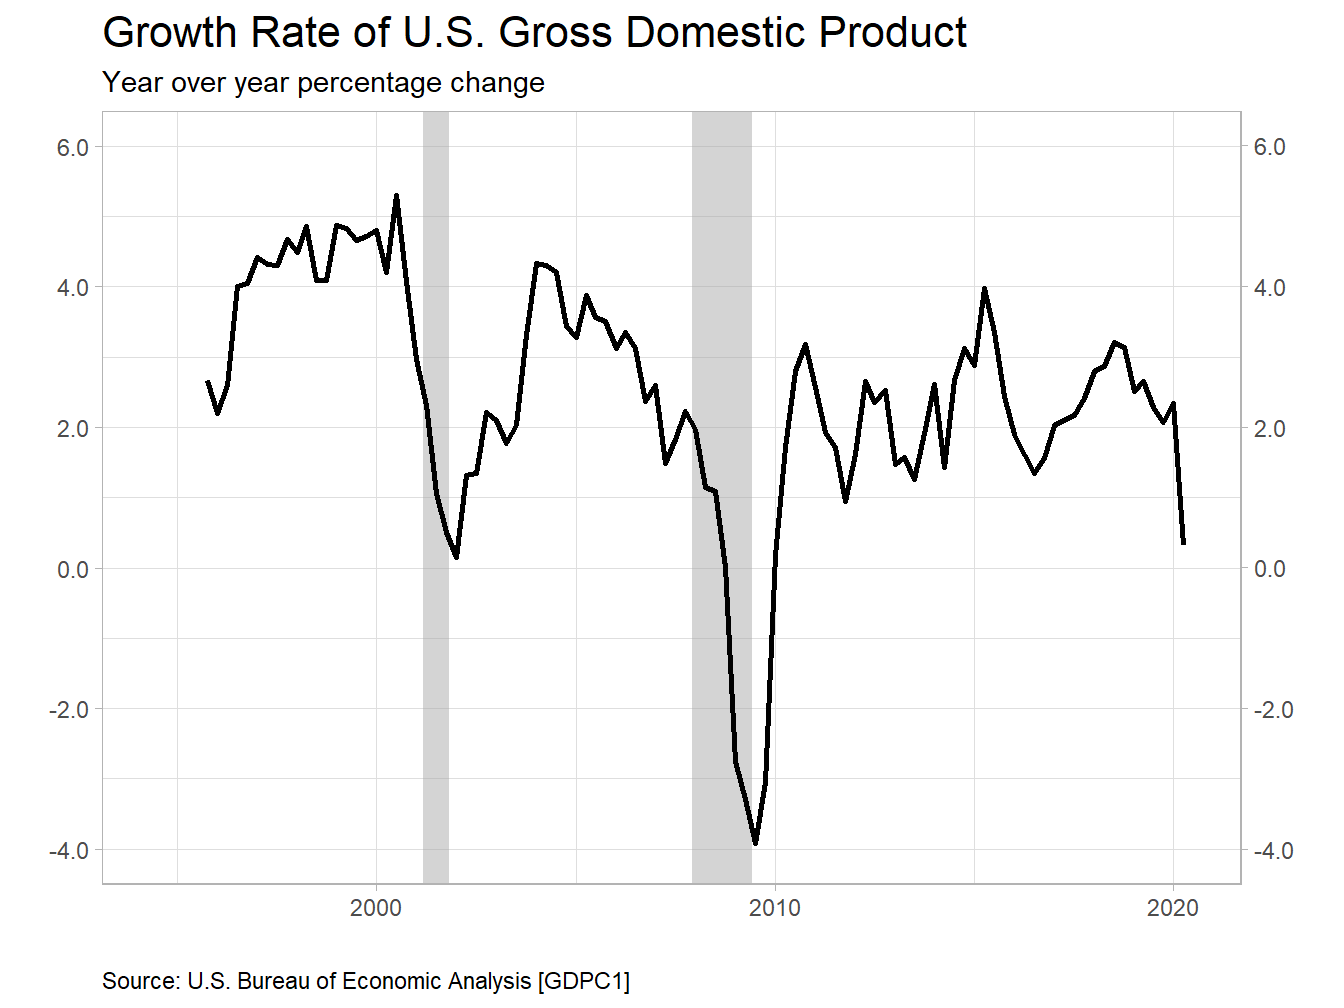
\includegraphics[width=0.8\linewidth]{econ200-book_files/figure-latex/output2-1} 

}

\caption{Output Exhibits Both Growth and Cycles}\label{fig:output2}
\end{figure}

\begin{figure}

{\centering 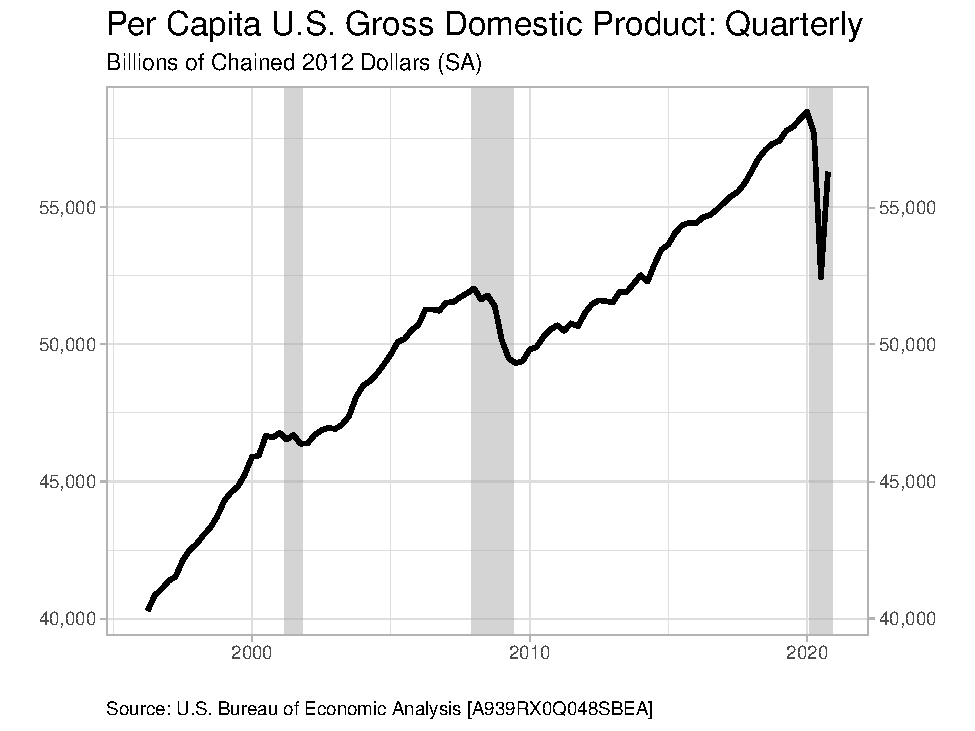
\includegraphics[width=0.8\linewidth]{econ200-book_files/figure-latex/output3-1} 

}

\caption{Per Capita GDP Might be More Important}\label{fig:output3}
\end{figure}

\begin{figure}

{\centering 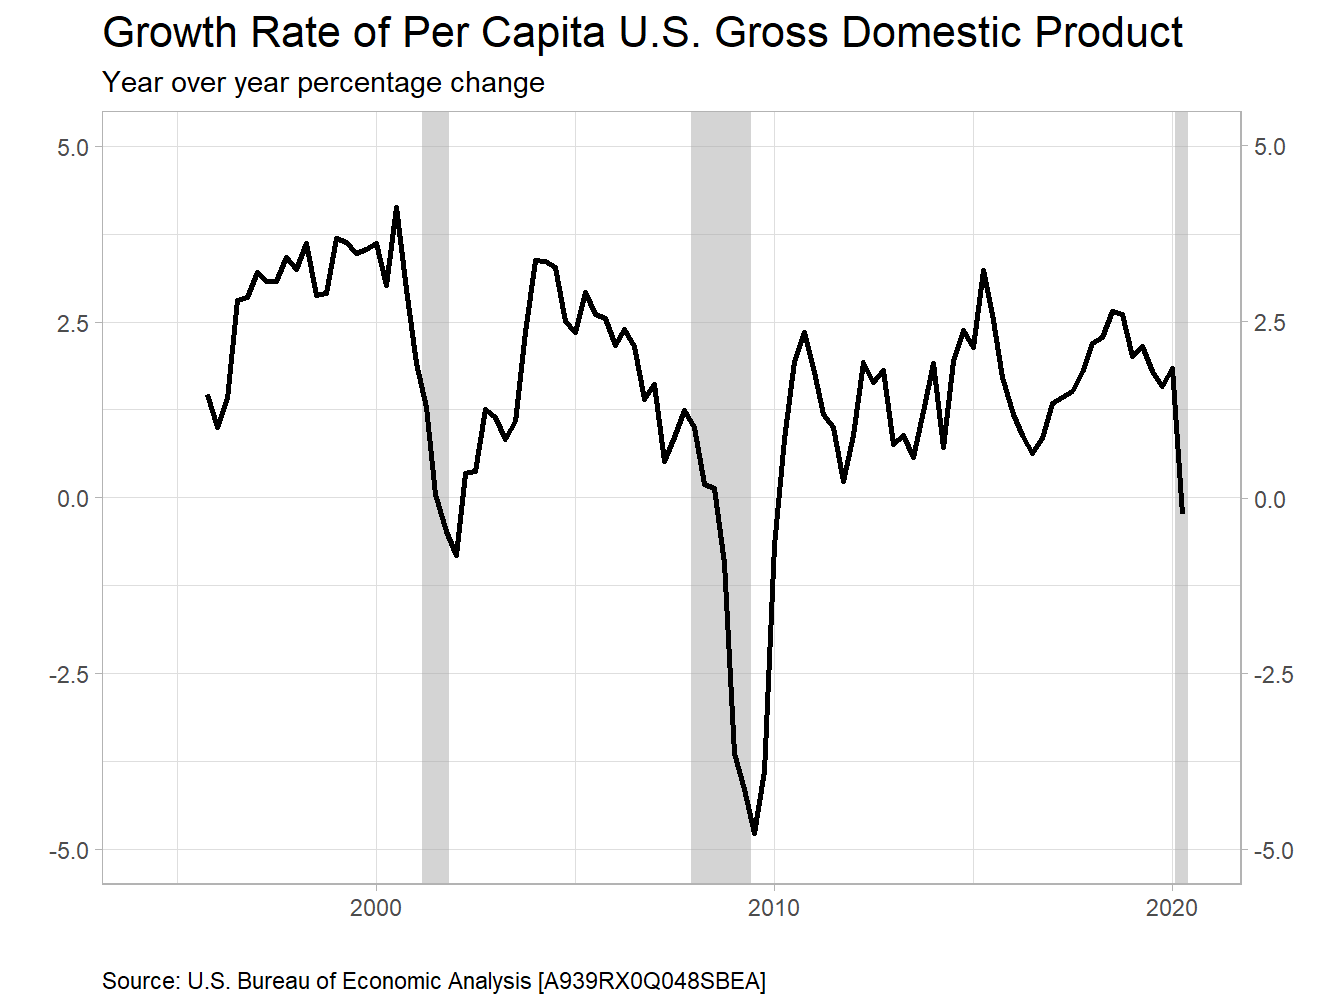
\includegraphics[width=0.8\linewidth]{econ200-book_files/figure-latex/output4-1} 

}

\caption{Per Capita Also Exhibits Cycles}\label{fig:output4}
\end{figure}

\begin{figure}

{\centering 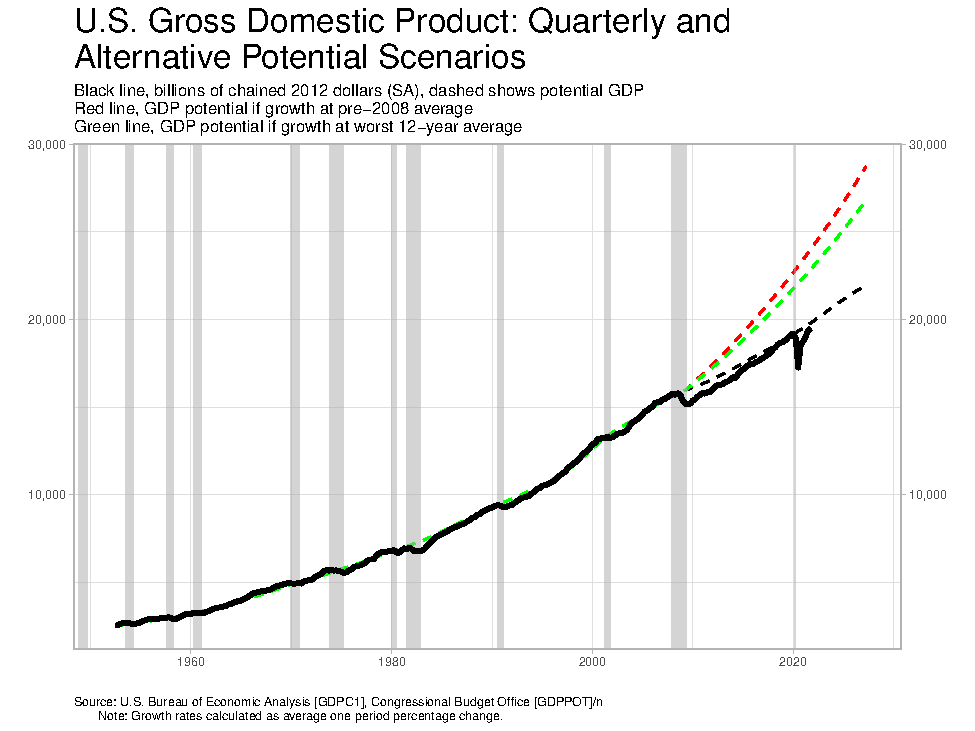
\includegraphics[width=0.8\linewidth]{econ200-book_files/figure-latex/output5-1} 

}

\caption{Per Capita Also Exhibits Cycles}\label{fig:output5}
\end{figure}

\begin{figure}

{\centering 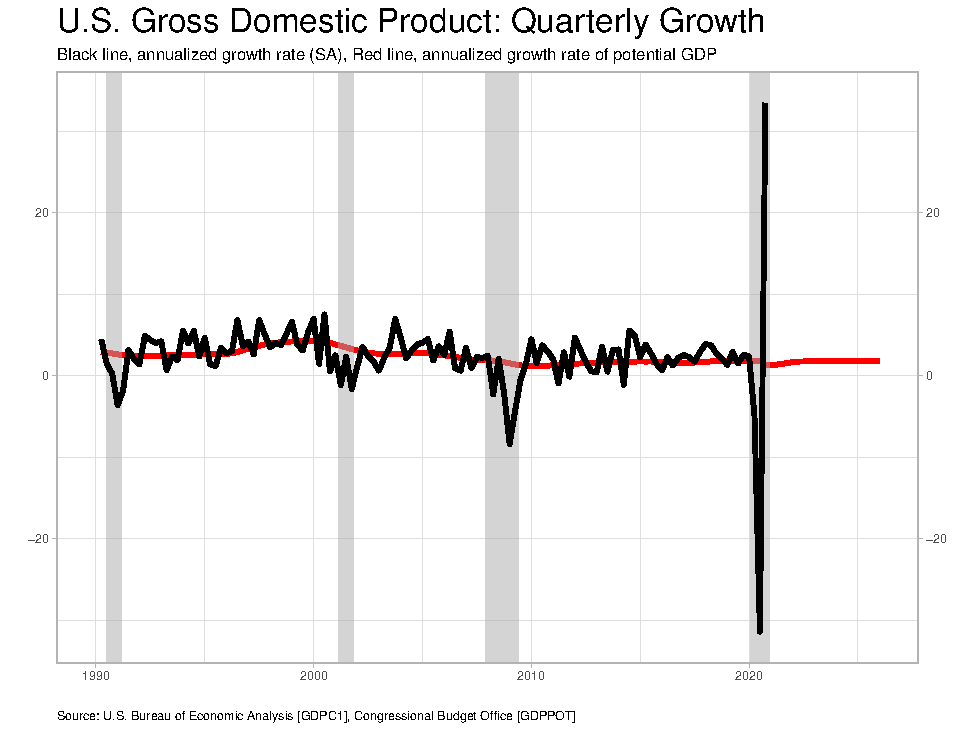
\includegraphics[width=0.8\linewidth]{econ200-book_files/figure-latex/output6-1} 

}

\caption{Per Capita Also Exhibits Cycles}\label{fig:output6}
\end{figure}

  \bibliography{refs.bib}

\end{document}
